%% LyX 2.3.3 created this file.  For more info, see http://www.lyx.org/.
%% Do not edit unless you really know what you are doing.
\documentclass[review]{elsarticle}
\usepackage[latin9]{inputenc}
\usepackage{array}
\usepackage{float}
\usepackage{units}
\usepackage{textcomp}
\usepackage{multirow}
\usepackage{amsmath}
\usepackage{amsthm}
\usepackage{graphicx}

\makeatletter

%%%%%%%%%%%%%%%%%%%%%%%%%%%%%% LyX specific LaTeX commands.
\DeclareTextSymbolDefault{\textquotedbl}{T1}
%% Because html converters don't know tabularnewline
\providecommand{\tabularnewline}{\\}
\floatstyle{ruled}
\newfloat{algorithm}{tbp}{loa}
\providecommand{\algorithmname}{Algorithm}
\floatname{algorithm}{\protect\algorithmname}

%%%%%%%%%%%%%%%%%%%%%%%%%%%%%% Textclass specific LaTeX commands.
\theoremstyle{plain}
\newtheorem{thm}{\protect\theoremname}
\theoremstyle{remark}
\newtheorem{rem}[thm]{\protect\remarkname}
\theoremstyle{definition}
\newtheorem{defn}[thm]{\protect\definitionname}
\theoremstyle{definition}
\newtheorem{example}[thm]{\protect\examplename}

%%%%%%%%%%%%%%%%%%%%%%%%%%%%%% User specified LaTeX commands.


%\usepackage{lineno}
%\modulolinenumbers[5]

\journal{Journal of Artificial Intelligence}

\usepackage{times}
\usepackage{latexsym}
\usepackage[algo2e]{algorithm2e} 


\usepackage{color}
\usepackage{units}
\usepackage{comment}


% Recommended, but optional, packages for figures and better typesetting:
\usepackage{graphicx}
\usepackage{subfigure}
\usepackage{booktabs}% for professional tables


%%%%%%%%%%%%%%%%%%%%%%%
%% Elsevier bibliography styles
%%%%%%%%%%%%%%%%%%%%%%%
%% To change the style, put a % in front of the second line of the current style and
%% remove the % from the second line of the style you would like to use.
%%%%%%%%%%%%%%%%%%%%%%%

%% Numbered
%\bibliographystyle{model1-num-names}

%% Numbered without titles
%\bibliographystyle{model1a-num-names}

%% Harvard
%\bibliographystyle{model2-names.bst}\biboptions{authoryear}

%% Vancouver numbered
%\usepackage{numcompress}\bibliographystyle{model3-num-names}

%% Vancouver name/year
%\usepackage{numcompress}\bibliographystyle{model4-names}\biboptions{authoryear}

%% APA style
%\bibliographystyle{model5-names}\biboptions{authoryear}

%% AMA style
%\usepackage{numcompress}\bibliographystyle{model6-num-names}

%% `Elsevier LaTeX' style

%%%%%%%%%%%%%%%%%%%%%%%

\makeatother

\providecommand{\definitionname}{Definition}
\providecommand{\examplename}{Example}
\providecommand{\remarkname}{Remark}
\providecommand{\theoremname}{Theorem}

\begin{document}
\begin{frontmatter}

\title{Learning to Play Two-Player Perfect-Information Games without Knowledge}

\author[mymainaddress]{Quentin Cohen-Solal}

\address[mymainaddress]{CRIL, Univ. Artois and CNRS, F-62300 Lens, France\\
LAMSADE, Universit� Paris-Dauphine, PSL, CNRS, France}

\ead[url]{cohen-solal@cril.fr}
\begin{abstract}
In this paper, several techniques for learning game state evaluation
functions by reinforcement are proposed. The first is a generalization
of tree bootstrapping (tree learning): it is adapted to the context
of reinforcement learning without knowledge based on non-linear functions.
With this technique, no information is lost during the reinforcement
learning process. The second is a modification of minimax with unbounded
depth extending the best sequences of actions to the terminal states.
This modified search is intended to be used during the learning process.
The third is to replace the classic gain of a game ($+1$ / $-1$)
with a \emph{reinforcement heuristic}. We study particular reinforcement
heuristics such as: quick wins and slow defeats ; scoring ; mobility
or presence. The fourth is another variant of unbounded minimax, which
plays the safest action instead of playing the best action. This modified
search is intended to be used after the learning process. The fifth
is a new action selection distribution. The conducted experiments
suggest that these techniques improve the level of play. We apply
these different techniques to design program-players to the game of
Hex (size $11$ and $13$) surpassing the level of Mohex 3HNN with
reinforcement learning from self-play without knowledge.   
\end{abstract}
\begin{keyword}
Machine Learning\sep Tree Search\sep Games\sep Game Tree Learning\sep
Minimax\sep Heuristic\sep Action Distribution\sep Unbound Minimax\sep
Hex.
\end{keyword}
\end{frontmatter}

\global\long\def\terminalrandom{\mathrm{t_{r}}}%
\global\long\def\hfb{\mathrm{b_{t}}}%
\global\long\def\hfp{\mathrm{p_{t}}}%
\global\long\def\hadapt{f_{\theta}}%
\global\long\def\hadaptnum#1{f_{\theta_{#1}}}%
\global\long\def\itreeset{\mathbf{T_{i}}}%
\global\long\def\treeset{\mathbf{T}}%
\global\long\def\rootset{\mathbf{R}}%
\global\long\def\hterminal{f_{\mathrm{t}}}%
\global\long\def\rnap{\mathrm{p_{rna}}}%
\global\long\def\rnab{\mathrm{b_{rna}}}%
\global\long\def\ubfm{\mathrm{UBFM}}%
\global\long\def\ubfmt{\ubfm_{\mathrm{s}}}%
\global\long\def\argmax{\operatorname*{\mathrm{arg\,max}}}%
\global\long\def\argmin{\operatorname*{\mathrm{arg\,min}}}%
\global\long\def\liste#1#2{\left\{  #1\,|\,#2\right\}  }%
\global\long\def\fterminal{\hterminal}%
\global\long\def\fadapt{\hadapt}%
\global\long\def\id{\mathrm{ID}}%
\global\long\def\minimum{\operatorname*{\mathrm{min}}}%


\section{Introduction}

One of the most difficult tasks in artificial intelligence is the
\emph{sequential decision making problem} \citep{littman1996algorithms},
whose applications include robotics and games. As for games, the successes
are numerous. Machine surpasses man for several games, such as backgammon,
checkers, chess, and go \citep{silver2017mastering}. A major class
of games is the set of two-player games in which players play in turn,
without any chance or hidden information. This class is sometimes
called two-player \emph{perfect information}\footnote{With some definitions, perfect information games include games with
chance. It depends on whether one includes information about the future
in perfect knowledge.} games \citet{mycielski1992games} or also two-player combinatorial
games. There are still many challenges for these games. For example,
for the \emph{game of Hex}, computers have only been able to beat
strong humans since 2020~\citep{cazenave2020polygames}. For \emph{general
game playing} \citep{genesereth2005general} (even restricted to games
with perfect information): man is always superior to machine on an
unknown complex game (when man and machine have a relatively short
learning time to master the rules of the game). In this article, we
focus on two-player zero-sum games with perfect information, although
most of the contributions in this article should be applicable or
easily adaptable to a more general framework\footnote{All the proposed techniques are directly applicable to the framework
of perfect information single-agent sequential decision-making problems
and in particular to solitaire games with perfect information. Tree
learning, ordinal distribution, and reinforcement heuristics are applicable
in the generalized cases (in case of $m$ agents, reinforcement heuristics
can be valued in real $m$-space). Minimax variants are applicable
in multi-player perfect-information games as variants of the paranoid
algorithm \citep{sturtevant2000pruning}. Descent can be applied to
learn value functions for stochastic perfect-information games by
applying it to a large set of determinist games corresponding to the
stochastic game where the chance was fixed and known before the start
of the game. To use the corresponding learned heuristic, either a
minimax at depth $1$ or an algorithm such as expectiminimax~\citep{michie1966game}
must be used. However, for stochastic games and multiplayer games
generalizations of the minimax variants should give better results
in general.}.

The first approaches used to design a game-playing program are based
on a game tree search algorithm, such as \emph{minimax}, combined
with a handcrafted game state evaluation function based on expert
knowledge. A notable use of this technique is the Deep Blue chess
program \citep{campbell2002deep}. However, the success of Deep Blue
is largely due to the raw power of the computer, which could analyze
two hundred million game states per second. In addition, this approach
is limited by having to design an evaluation function manually (at
least partially). This design is a very complex task, which must,
in addition, be carried out for each different game. Several works
have thus focused on the automatic learning of evaluation functions
\citep{mandziuk2010knowledge}. One of the first successes of learning
evaluation functions is on the Backgammon game \citep{tesauro1995temporal}.
However, for many games, such as Hex or Go, minimax-based approaches,
with or without machine learning, have failed to overcome human. Two
causes have been identified \citep{baier2018mcts}. Firstly, the
very large number of possible actions at each game state prevents
an exhaustive search at a significant depth (the game can only be
anticipated a few turns in advance). Secondly, for these games, no
sufficiently powerful evaluation function could be identified. An
alternative approach to solve these two problems has been proposed,
giving notably good results to Hex and Go, called Monte Carlo Tree
Search and denoted MCTS \citep{Coulom06,browne2012survey}. This
algorithm explores the game tree non-uniformly, which is a solution
to the problem of the very large number of actions. In addition, it
evaluates the game states from victory statistics of a large number
of random end-game simulations. It does not need an evaluation function.
This was not enough, however, to go beyond the level of human players.
Several variants of Monte Carlo tree search were then proposed, using
in particular knowledge to guide the exploration of the game tree
and/or random end-game simulations \citep{browne2012survey}. Recent
improvements in Monte Carlo tree research have focused on the automatic
learning of MCTS knowledge and their uses. This knowledge was first
generated by \emph{supervised learning} \citep{clark2015training,gao2017move,gao2018three,cazenave2018residual,tian2015better}
then by supervised learning followed by \emph{reinforcement learning}
\citep{silver2016mastering}, and finally by only reinforcement learning
\citep{silver2017mastering,anthony2017thinking,silver2018general}.
This allowed programs to reach and surpass the level of world champion
at the game of Go with the latest versions of the program AlphaGo
\citep{silver2016mastering,silver2017mastering}. In particular, AlphaGo
zero \citep{silver2017mastering}, which only uses reinforcement learning,
did not need any knowledge to reach its level of play. This last success,
however, required 29 million games of self-play (with 1,600 state
evaluations per move). This approach has also been applied to chess
\citep{silver2017mastering2}. The resulting program broke the best
chess program (which is based on minimax). AlphaZero was subsequently
reimplemented in Polygames \citep{cazenave2020polygames}, an open-source
and multi-game program, which was notably applied to Hex and Havannah.
In particular, at the 2020 Computer Olympiad, the gold medals for
these games were won by Polygames.

It is therefore questionable whether minimax is totally out of date
or whether the spectacular successes of recent programs are more based
on reinforcement learning than Monte Carlo tree search. In particular,
it is interesting to ask whether reinforcement learning would enhance
minimax enough to make it competitive with Monte Carlo tree search
on games where it dominates minimax so far, such as Go or Hex.

In this article\footnote{Note that this paper is an extended, improved, and english version
of~\citep{cohen2019apprendre}.}, we therefore focus on reinforcement learning within the minimax
framework. We propose and asses new techniques for reinforcement learning
of evaluation functions. Then, we apply them to design new program-players
to the game of Hex (without using other knowledge than the rules of
the game). We compare this program-player to Mohex 3HNN \citep{gao2018three},
the best Hex program, champion at Hex (size 11 and 13) of the $2018$
Computer Olympiad \citep{gao2019hex}. 

In the next section, we briefly present the game algorithms and in
particular minimax with unbounded depth on which we base several of
our experiments. We also present reinforcement learning in games,
the game of Hex, the state of the art of game programs on this game,
as well as other games on which experiments are performed. In the
following sections, we propose different techniques aimed at improving
learning performances and we expose the experiments carried out using
these techniques. In particular, in Section~\ref{sec:Data-Usage},
we extends the tree bootstrapping (tree learning) technique to the
context of reinforcement learning without knowledge based on non-linear
functions. In Section~\ref{sec:Search-Algorithms-for-Learning},
we present a new search algorithm, a variant of unbounded minimax
called \emph{descent}, intended to be used during the learning process.
In Section~\ref{sec:Reinforcement-Heuristic}, we introduce reinforcement
heuristics. Their usage is a simple way to use general or dedicated
knowledge in reinforcement learning processes. We study several reinforcement
heuristics in the context of different games. In Section~\ref{sec:Search-Algorithms-for-Playing},
we propose another variant of unbounded minimax, which plays the safest
action instead of playing the best action. This modified search is
intended to be used after the learning process. In Section~\ref{sec:Ordinal-Distribution-and-Application},
we introduce a new action selection distribution and we apply it with
all the previous techniques to design program-players to the game
of Hex (size 11 and 13) and compare them to Mohex 3HNN.    Finally,
in the last section, we conclude and expose the different research
perspectives.

\section{Background and Related Work\label{sec:RW}}

In this section, we briefly present game tree search algorithms, reinforcement
learning in the context of games and their applications to Hex and
Chess (for more details about game algorithms, see \citep{yannakakis2018artificial}).

Games can be represented by their \emph{game tree} (a node corresponds
to a game state and the children of a node are the states that can
be reached by an action). From this representation, we can determine
the action to play using a game tree search algorithm. In order to
win, each player tries to maximize his score (i.e. the value of the
game state for this player at the end of the game). As we place ourselves
in the context of two-player zero-sum games, to maximize the score
of a player is to minimize the score of his opponent (the score of
a player is the negation of the score of his opponent).

\subsection{Game Tree Search Algorithms}

The central algorithm is \emph{minimax} which recursively determines
the value of a node from the value of its children and the functions
$\min$ and $\max$, up to a limit recursion depth. With this algorithm,
the game tree is uniformly explored. A better implementation of minimax
uses \emph{alpha-beta pruning} \citep{knuth1975analysis,yannakakis2018artificial}
which makes it possible not to explore the sections of the game tree
which are less interesting given the values of the nodes already met
and the properties of $\min$ and $\max$. Many variants and improvements
of minimax have been proposed \citep{millington2009artificial}. For
instance, \emph{iterative deepening} \citep{slate1983chess,korf1985depth}
allows one to use minimax with a time limit. It sequentially performs
increasing depth alpha-beta searches as long as there is time. It
is generally combined with the \emph{move ordering} technique \citep{fink1982enhancement},
which consists of extending the best move from the previous search
first, which accelerates the new search. Some variants perform a search
with unbounded depth (that is, the depth of their search is not fixed)
\citep{van2008proof,schaeffer1990conspiracy,berliner1981b}. Unlike
minimax with or without alpha-beta pruning, the exploration of these
algorithms is non-uniform. One of these algorithms is the\emph{ best-first
minimax search }\citep{korf1996best}. To avoid any confusion with
some best-first approaches at fixed depth, we call this algorithm
\emph{Unbound Best-First Minimax}, or more succinctly $\ubfm$. $\ubfm$
iteratively extends the game tree by adding the children of one of
the leaves of the game tree having the same value as that of the root
(minimax value). These leaves are the states obtained after having
played one of the best sequences of possible actions given the current
partial knowledge of the game tree. Thus, this algorithm iteratively
extends the \emph{a priori} best sequences of actions. These best
sequences usually change at each extension. Thus, the game tree is
non-uniformly explored by focusing on the \emph{a priori} most interesting
actions without exploring just one sequence of actions. In this article,
we use the anytime version of $\ubfm$ \citep{korf1996best}, i.e.
we leave a fixed search time for $\ubfm$ to decide the action to
play. We also use transposition tables \citep{greenblatt1988greenblatt,millington2009artificial}
with $\ubfm$, which makes it possible not to explicitly build the
game tree and to merge the nodes corresponding to the same state.
Algorithm~\ref{alg:-Unbounded-Best-First-Mininmax} is the used implementation
of $\ubfm$ in this paper\footnote{This implementation is a slight variant of Korf and Chickering algorithm.
Their algorithm is very slightly more efficient but it offers less
freedom: our algorithm behaves slightly differently depending on how
we decide between two states having the same value. The exploration
of states is identical between their algorithm and ours when with
our algorithm equality is decided in deepest first. Our variant has
been discovered independently of Korf and Chickering work.}. 
\begin{table}
\begin{centering}
{\footnotesize{}}%
\begin{tabular}{|c|c|}
\hline 
{\footnotesize{}Symbols} & {\footnotesize{}Definition}\tabularnewline
\hline 
\hline 
{\footnotesize{}$\mathrm{actions}\left(s\right)$} & {\footnotesize{}action set of the state $s$ for the current player}\tabularnewline
\hline 
{\footnotesize{}$\mathrm{first\_player}\left(s\right)$} & {\footnotesize{}true if the current player of the state $s$ is the
first player}\tabularnewline
\hline 
{\footnotesize{}$\mathrm{terminal\left(s\right)}$} & {\footnotesize{}true if $s$ is an end-game state}\tabularnewline
\hline 
{\footnotesize{}$a(s)$} & {\footnotesize{}state obtained after playing the action $a$ in the
state $s$}\tabularnewline
\hline 
{\footnotesize{}$\mathrm{time}\left(\right)$} & {\footnotesize{}current time in seconds}\tabularnewline
\hline 
{\footnotesize{}$S$} & {\footnotesize{}keys of the transposition table $T$}\tabularnewline
\hline 
{\footnotesize{}$T$} & {\footnotesize{}transposition table (contains functions as $v$ and/or
$v'$ ; depends on the used search algorithm)}\tabularnewline
\hline 
{\footnotesize{}$\tau$} & {\footnotesize{}search time per action}\tabularnewline
\hline 
{\footnotesize{}$t$} & {\footnotesize{}time elapsed since the start of the reinforcement
learning process}\tabularnewline
\hline 
{\footnotesize{}$t_{\max}$} & {\footnotesize{}chosen total duration of the learning process }\tabularnewline
\hline 
{\footnotesize{}$n(s,a)$} & {\footnotesize{}number of times the action $a$ is selected in state
$s$ (initially, $n(s,a)=0$ for all $s$ and $a$}\tabularnewline
\hline 
{\footnotesize{}$v(s)$} & {\footnotesize{}value of state $s$ in the game tree according to
the last tree search}\tabularnewline
\hline 
{\footnotesize{}$v'(s,a)$} & {\footnotesize{}value obtained after playing action $a$ in state
$s$}\tabularnewline
\hline 
{\footnotesize{}$c(s)$} & {\footnotesize{}completion value of state $s$ ($0$ by default)}\tabularnewline
\hline 
{\footnotesize{}$r(s)$} & {\footnotesize{}resolution value of state $s$ ($0$ by default)}\tabularnewline
\hline 
{\footnotesize{}$f(s)$} & {\footnotesize{}the used evaluation function (first player point of
view)}\tabularnewline
\hline 
{\footnotesize{}$\hadapt(s)$} & {\footnotesize{}adaptive evaluation function (of non-terminal game
tree leaves ; first player point of view)}\tabularnewline
\hline 
{\footnotesize{}$\hterminal(s)$} & {\footnotesize{}evaluation of terminal states, e.g. gain game (first
player point of view)}\tabularnewline
\hline 
{\footnotesize{}Gain function $\hfb(s)$} & {\footnotesize{}$0$ if $s$ is a draw, $1$ if $s$ is winning for
the first player, $-1$ if $s$ is losing for the first player}\tabularnewline
\hline 
\multirow{3}{*}{{\footnotesize{}search($s$, $S$, $T$, $\hadapt$, $\hterminal$)}} & {\footnotesize{}a seach algorithm (it extends the game tree from $s$,
by adding new states in $S$ }\tabularnewline
 & {\footnotesize{}and labeling its states, in particular, by a value
$v(s)$, stored in $T$, }\tabularnewline
 & {\footnotesize{}using $\hadapt$ as evaluation of the non-terminal
leaves and $\hterminal$ as evaluation of terminal states}\tabularnewline
\hline 
{\footnotesize{}action\_selection($s$, $S$, $T$)} & {\footnotesize{}decides the action to play in the state $s$ depending
on the partial game tree, i.e. on $S$ and $T$}\tabularnewline
\hline 
{\footnotesize{}processing($D$)} & {\footnotesize{}various optional data processing: data augmentation
(symmetry), experience replay, ... }\tabularnewline
\hline 
{\footnotesize{}update($\hadapt,D$)} & {\footnotesize{}updates the parameter $\theta$ of $\hadapt$ in order
for $\hadapt(s)$ is closer to $v$ for each $(s,v)\in D$}\tabularnewline
\hline 
\end{tabular}{\footnotesize\par}
\par\end{centering}
\caption{Index of symbols\label{tab:Index-of-symbols}}
\end{table}

\begin{algorithm}
\DontPrintSemicolon\SetAlgoNoEnd
\SetKwFunction{iterationUM}{UBFM\_iteration}
\SetKwFunction{UM}{UBFM}\SetKwFunction{time}{time}\SetKwFunction{actions}{actions}\SetKwFunction{bestaction}{best\_action}\SetKwFunction{terminal}{terminal}\SetKwFunction{premier}{first\_player} \SetKwProg{myproc}{Function}{}{}
\myproc{\iterationUM{$s$, $S$, $T$}}{
\eIf{\terminal{$s$}}{return $f(s)$}{
\eIf{$s\notin S$}{
$S\leftarrow S\cup\{s\}$\;

\ForEach{$a\in$ \actions{$s$}}{$v'(s,a)\leftarrow f\left(a(s)\right)$\; }
}{
$a_{b}\leftarrow$ \bestaction{$s$}\;

$v'(s,a_{b})\leftarrow$ \iterationUM{$a_{b}(s)$, $S$, $T$}\;

} 

$a_{b}\leftarrow$ \bestaction{$s$}\; 

return $v'(s,a_{b})$\;
}
}
\;
\myproc{\bestaction{$s$, $S$, $T$}}{
\eIf{\premier{$s$}}{return ${\displaystyle \argmax_{a\in\actions{s}}v'\left(s,a\right)}$\;}{
return ${\displaystyle \argmin_{a\in\actions{s}}v'\left(s,a\right)}$\;
}
}
\;
\myproc{\UM{$s$, $\tau$}}{
$t=$ \time{}\;
\lWhile{\time{}$-\,t<\tau$}{\iterationUM{$s$, $S$, $T$}}
return \bestaction{$s$, $S$, $T$}\;
}\;

\caption{$\protect\ubfm$ (Unbounded Best-First Minimax) algorithm : it computes
the best action to play in the generated non-uniform partial game
tree (see Table~\ref{tab:Index-of-symbols} for the definitions of
symbols ; at any time $T=\protect\liste{v'(s,a)}{s\in S,a\in\mathrm{actions}(s)}$).\label{alg:-Unbounded-Best-First-Mininmax}}
\end{algorithm}


\subsection{Learning of Evaluation Functions\label{subsec:RW-Apprentissage-de-fonctions}}

Reinforcement learning of evaluation functions can be done by different
techniques \citep{mandziuk2010knowledge,silver2017mastering,anthony2017thinking,young2016neurohex}.
The general idea of reinforcement learning of state evaluation functions
is to use a game tree search algorithm and an adaptive evaluation
function $\hadapt$, of parameter $\theta$, (for example a neural
network) to play a sequence of games (for example against oneself,
which is the case in this article). Each game will generate pairs
$(s,v)$ where $s$ is a state and $v$ the value of $s$ calculated
by the chosen search algorithm using the evaluation function $\hadapt$.
The states generated during one game can be the states of the sequence
of states of the game \citep{tesauro1995temporal,veness2009bootstrapping}.
For example, in the case of \emph{root bootstrapping} (technique that
we call \emph{root learning} in this article), the set of pairs used
during the learning phase is $D=\liste{\left(s,v\right)}{s\in\rootset}$
with $\rootset$ the set of states of the sequence of the game. In
the case of the \emph{tree bootstrapping} (\emph{tree learning}) technique
\citep{veness2009bootstrapping}, the generated states are the states
of the game tree built to decide which actions to play (which includes
the states of the sequence of states of the game): $D=\liste{\left(s,v\right)}{s\in\treeset}$
with $\treeset$ the set of states of the partial game tree of the
game. Thus, contrary to root bootstrapping, tree bootstrapping does
not discard most of the information used to decide the actions to
play. The values of the generated states can be their minimax values
in the partial game tree built to decide which actions to play~\citep{veness2009bootstrapping,tesauro1995temporal}.
Work on tree bootstrapping has been limited to reinforcement learning
of linear functions of state features. It has not been formulated
or studied in the context of reinforcement learning without knowledge
and based on non-linear functions. Note that, in the case of AlphaGo
Zero, the value of each generated state, the states of the sequence
of the game, is the value of the terminal state of the game \citep{silver2017mastering}.
We call this technique terminal learning. 

Generally between two consecutive games (between \emph{match phases}),
a \emph{learning phase} occurs, using the pairs of the last game.
Each learning phase consists in modifying $\hadapt$ so that for all
pairs $(s,v)\in D$, $\hadapt(s)$ sufficiently approaches $v$ to
constitute a good approximation. Note that, in the context of a variant,
learning phases can use the pairs of \emph{several} games. This technique
is called \emph{experience replay} \citep{mnih2015human}. Note that,
adaptive evaluation functions $\hadapt$ only serve to evaluate non-terminal
states since we know the true value of terminal states. 
\begin{rem}
There is another reinforcement learning technique for games: the Temporal
Differences differences $\mathrm{TD}(\lambda)$~\citep{tesauro1995temporal}.
We can see the temporal differences as a kind of interpolation between
root learning of a depth $1$ minimax and the terminal learning. A
variant has been proposed~\citep{baxter2000learning}, called $\mathrm{TD_{Leaf}}(\lambda)$,
where the temporal difference technique is applied not to learn the
value of the root but the value of the leaf of the principal variation
of a minimax search (at any depth). A comparison between these techniques
was made~\citep{veness2009bootstrapping}. Finally, \citep{bjornsson2003learning}
describe a method for automatically tuning search-extension parameters,
to decide which branches of the game tree must be explored during
the search.
\end{rem}


\subsection{Action Selection Distribution\label{subsec:Distribution-de-s=00003D0000E9lection}}

One of the problems related to reinforcement learning is the \emph{exploration-exploitation
dilemma} \citep{mandziuk2010knowledge}. It consists of choosing between
exploring new states to learn new knowledge and exploiting the acquired
knowledge. Many techniques have been proposed to deal with this dilemma
\citep{mellor2014decision}. However, most of these techniques do
not scale because their application requires memorizing all the encountered
states. For this reason, in the context of games with large numbers
of states, some approaches use probabilistic exploration \citep{young2016neurohex,silver2017mastering,mandziuk2010knowledge,schraudolph2001learning}.
With this approach, to exploit is to play the best action and to explore
is to play uniformly at random. More precisely, a parametric probability
distribution is used to associate with each action its probability
of being played. The parameter associated with the distribution corresponds
to the exploration rate (between $0$ and $1$), which we denote $\epsilon$
(the exploitation rate is therefore $1-\epsilon$, which we denote
$\epsilon'$). The rate is often experimentally fixed. \emph{Simulated
annealing} \citep{kirkpatrick1983optimization} can, however, be applied
to avoid choosing a value for this parameter. In this case, at the
beginning of reinforcement learning, the parameter is $1$ (we are
just exploring). It gradually decreases until reaching $0$ at the
end of learning. The simplest action selection distribution is \emph{$\epsilon$-greedy}
\citep{young2016neurohex} (of parameter $\epsilon$). With this distribution,
the action is chosen uniformly with probability $\epsilon$ and the
best action is chosen with probability $1-\epsilon$ (see also Algorithm~\ref{alg:e-greedy}). 

\begin{algorithm}[!bh]
\DontPrintSemicolon\SetAlgoNoEnd

\SetKwFunction{egreedy}{$\epsilon$\_greedy}\SetKwFunction{actions}{actions}\SetKwFunction{premier}{first\_player}\SetKwProg{myproc}{Function}{}{}

\myproc{\egreedy{$s$, $v'$}}{

\eIf{probability $\frac{t}{t_{\max}}$ }{

\eIf{\premier{$s$}}{

return $\argmax_{a\in\text{\actions{\text{s}}}}v'\left(s,a\right)$
\;

}{

return $\argmin_{a\in\text{\actions{\text{s}}}}v'\left(s,a\right)$
\;

}

}{

return $a\in\text{\actions{\text{s}}}$ uniformly chosen.\;

}

}\;

\protect\protect

\caption{$\epsilon$-greedy algorithm with simulated annealing used in the
experiments of this article (see Table~\ref{tab:Index-of-symbols}
for the definitions of symbols).\label{alg:e-greedy}}
\end{algorithm}
The $\epsilon$-greedy distribution has the disadvantage of not differentiating
the actions (except the best action) in terms of probabilities. Another
distribution is often used, correcting this disadvantage. This is
the \emph{softmax} distribution \citep{schraudolph2001learning,mandziuk2010knowledge}.
It is defined by $P\left(a_{i}\right)=\frac{e^{\nicefrac{v'(s,a_{i})}{\tau}}}{\sum_{j=1}^{n}e^{\nicefrac{v'(s,a_{j})}{\tau}}}$
with $n$ the number of children of the current state $s$, $P\left(a_{i}\right)$
the probability of playing the action $a_{i}$ , $v'(s,a_{i})$ the
value of the state obtained after playing $a_{i}$ in $s$, $i\in\{0,\ldots,n-1\}$,
and $\tau\in]0,+\infty[$ a parameter called temperature ($\tau\simeq0$
: exploitation, $\tau\simeq+\infty$ : exploration).

\subsection{Game of Hex}

The game of Hex \citep{browne2000hex} is a two-player combinatorial
strategy game. It is played on an empty $n\times n$ hexagonal board.
We say that a $n\times n$ board is of size $n$. The board can be
of any size, although the classic sizes are $11$, $13$ and $19$.
In turn, each player places a stone of his color on an empty cell
(each stone is identical). The goal of the game is to be the first
to connect the two opposite sides of the board corresponding to its
color. Figure~\ref{fig:Fin-de-partie} illustrates an end game. Although
these rules are simplistic, Hex tactics and strategies are complex.
The number of states and the number of actions per state are very
large, similar to the game of Go. From the board size $11$, the number
of states is, for example, higher than that of chess (Table~$6$
of \citep{van2002games}). For any board size, the first player has
a winning strategy \citep{berlekamp2018winning} which is unknown,
except for board sizes smaller than or equal to $10$ \citep{pawlewicz2013scalable}
(the game is weaky solved up to the size $10$). In fact, resolving
a particular state is PSPACE-complete \citep{reisch1981hex,bonnet2016complexity}.
There is a variant of Hex using a swap rule. With this variant, the
second player can play in first action a special action, called swap,
which swaps the color of the two players (i.e. they swap their pieces
and their sides). This rule reduces the imbalance between the two
players (without the swap rule, the first player has a very strong
advantage). It is generally used in competitions.

\begin{figure}[t]
\begin{centering}
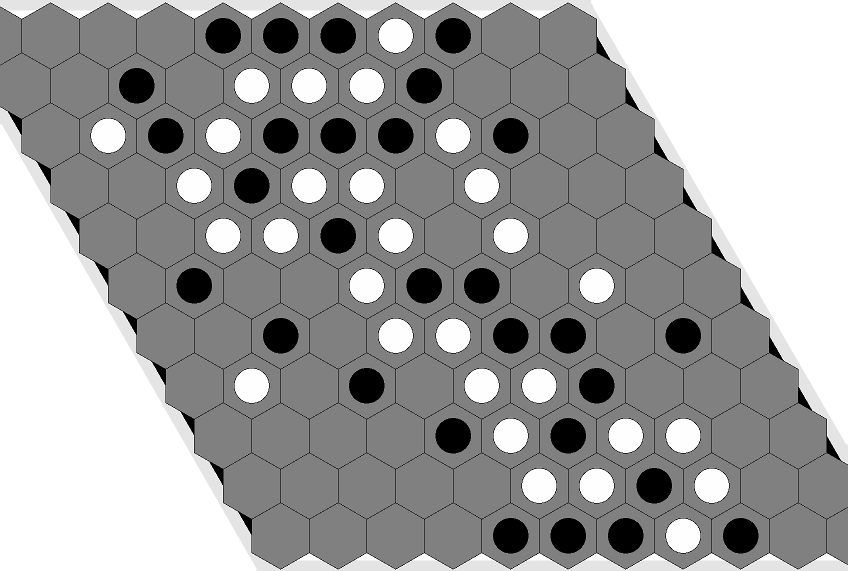
\includegraphics[scale=0.2]{image_hex_2}
\par\end{centering}
\centering{}\caption{A Hex end game of size 11 (white wins)\label{fig:Fin-de-partie}}
\end{figure}


\subsection{Hex Programs\label{subsec:Programmes-joueurs-au-Hex}}

Many Hex player programs have been developed. For example, Mohex 1.0
\citep{huang2013mohex} is a program based on Monte Carlo tree search.
It also uses many techniques dedicated to Hex, based on specific theoretical
results. In particular, it is able to quickly determine a winning
strategy for some states (without expanding the search tree) and to
prune at each state many actions that it knows to be \emph{inferior}.
It also uses ad hoc knowledge to bias simulations of Monte Carlo tree
search.

Mohex 2.0 \citep{huang2013mohex} is an improvement of Mohex 1.0 that
uses learned knowledge through supervised learning (namely correlations
between victory and board patterns) to guide both tree exploration
and simulations.

Other work then focused on predicting best actions, through supervised
learning of a database of games, using a neural network \citep{michalski2013machine,lecun2015deep,goodfellow2016deep}.
The neural network is used to learn a \emph{policy}, i.e. a prior
probability distribution on the actions to play. These prior probabilities
are used to guide the exploration of Monte Carlo tree search. First,
there is Mohex-CNN \citep{gao2017move} which is an improvement of
Mohex 2.0 using a convolutional neural network \citep{krizhevsky2012imagenet}.
A new version of Mohex was then proposed: Mohex-3HNN \citep{gao2018three}.
Unlike Mohex-CNN, it is based on a residual neural network \citep{he2016deep}.
It calculates, in addition to the policy, a value for states \emph{and}
actions. The value of states replaces the evaluation of states based
on simulations of Monte Carlo tree search. Adding a value to actions
allows Mohex-HNN to reduce the number of calls of the neural network,
improving performance. Mohex-3HNN is the best Hex program. It wons
Hex size 11 and 13 tournaments at 2018 Computer Olympiad \citep{gao2019hex}.

Programs which learn the evaluation function by reinforcement have
also been designed. These programs are NeuroHex \citep{young2016neurohex},
EZO-CNN \citep{takada2017reinforcement}, DeepEzo \citep{takada2019reinforcement}
and ExIt \citep{anthony2017thinking}. They learn from self-play.
Unlike the other three programs, NeuroHex performs supervised learning
(of a common Hex heuristic) followed by reinforcement learning. NeuroHex
also starts its games with a state from a database of games. EZO-CNN
and DeepEzo use knowledge to learn winning strategies in some states.
DeepEzo also uses knowledge during confrontations. ExIt learns a policy
in addition to the value of states and it is based on MCTS. It is
the only program to have learned to play Hex without using knowledge.
This result is, however, limited to the board size $9$. A comparison
of the main characteristics of these different programs is presented
in Table~\ref{tab:comparatif}.

\begin{table*}[t]
\begin{centering}
{\footnotesize{}{}}%
\begin{tabular}{|c|c|c|c|c|c|}
\hline 
{\footnotesize{}{}Programs} & {\footnotesize{}{}Size} & {\footnotesize{}{}Search} & {\footnotesize{}{}Learning} & {\footnotesize{}{}Network} & {\footnotesize{}{}Use}\tabularnewline
\hline 
\hline 
{\footnotesize{}{}Mohex-CNN} & {\footnotesize{}{}13} & {\footnotesize{}{}MCTS} & {\footnotesize{}{}supervised} & {\footnotesize{}{}convolutional} & {\footnotesize{}{}policy}\tabularnewline
\hline 
{\footnotesize{}{}Mohex-3HNN} & {\footnotesize{}{}13} & {\footnotesize{}{}MCTS} & {\footnotesize{}{}supervised} & {\footnotesize{}{}residual} & {\footnotesize{}{}policy, state, action}\tabularnewline
\hline 
{\footnotesize{}{}NeuroHex} & {\footnotesize{}{}13} & {\footnotesize{}{}none} & {\footnotesize{}{}supervised, reinforcement} & {\footnotesize{}{}convolutional} & {\footnotesize{}{}state}\tabularnewline
\hline 
{\footnotesize{}{}EZO-CNN} & {\footnotesize{}{}7, 9, 11} & {\footnotesize{}{}Minimax} & {\footnotesize{}{}reinforcement} & {\footnotesize{}{}convolutional} & {\footnotesize{}{}state}\tabularnewline
\hline 
{\footnotesize{}{}DeepEZO} & {\footnotesize{}{}13} & {\footnotesize{}{}Minimax} & {\footnotesize{}{}reinforcement} & {\footnotesize{}{}convolutional} & {\footnotesize{}{}policy, state}\tabularnewline
\hline 
{\footnotesize{}{}ExIt} & {\footnotesize{}{}9} & {\footnotesize{}{}MCTS} & {\footnotesize{}{}reinforcement} & {\footnotesize{}{}convolutional} & {\footnotesize{}{}policy, state}\tabularnewline
\hline 
\end{tabular}
\par\end{centering}
\caption{Comparison of the main features of the latest Hex programs. These
characteristics are respectively the board sizes on which learning
is based, the used tree search algorithm, the type of learning, the
type of neural network and its use (to approximate the values of states,
actions and/or policy.\label{tab:comparatif}}
\end{table*}


\subsection{Games of Paper Experiments}

We now briefly present the other games on which experiments are performed
in this article, namely: Surakarta, Othello, Outer Open Gomoku, Clobber,
Breakthrough, Amazons, Lines of Action, Santorini. They are all board
games. All of these games (except Santorini so far) are present and
recurring at the Computer Olympiads, the worldwide multi-games event
in which computer programs compete against each other. Moreover, all
these games (and their rules) are included (and available for free)
in Ludii~\citep{Piette2020Ludii}, a general game system. 

\subsubsection{Surakarta}

Surakarta is a move and capture game (like the checkers game), the
object of the game being to take all the opposing pieces. In his turn,
a player can either move a piece to an empty square at a distance
of $1$ or move a piece to a square occupied by an opponent's piece
under certain conditions and according to a mechanism specific to
Surakarta (based on a movement circuit dedicated only to capture),
allowing \textquotedbl long distance\textquotedbl{} capture.

\subsubsection{Othello}

Othello (also called Reversi) is a linear territory and encirclement
game whose goal is to have more pieces than your opponent. In his
turn, a player places a piece of his color on the board (only if he
can make an encirclement, otherwise he pass his turn). There is an
encirclement if an opponent's line of pieces has at its two ends the
piece that has just been placed and another piece of the player performing
the encirclement. As a result of this encirclement, the encircled
pieces are replaced by pieces from that player.

\subsubsection{Outer Open Gomoku}

Outer Open Gomoku is an alignment game. The object of the game is
to line up at least $5$ pieces of its color. On his turn, a player
places a piece of his color. In the first turn, the first player can
only place a piece at a distance of $2$ from the sides of the board.

\subsubsection{Clobber}

Clobber is a move and capture game. The goal is to be the last player
to have played. A player can play if he can orthogonally move one
of his pieces onto a neighboring square on which there is an opponent's
piece. This movement is always a capture (the opponent's piece is
removed from the board).

\subsubsection{Breakthrough}

Breakthrough is a move and capture game. The object of the game is
to be the first to make one of his pieces reach the other side of
the board. A piece can only move by moving forward one square (straight
or diagonal). A capture can only be done diagonally.

\subsubsection{Amazons}

Amazons is a move and blocking game. In turn, a player moves one of
his pieces in a straight line in any direction (like the queen of
the game of Chess). Then he places a neutral piece (blocking movements
like the players' pieces) in any direction starting from the new position
of the piece just moved (in the manner of the queen of the game of
Chess). The goal of the game is to be the last to play.

\subsubsection{Lines of Action}

Lines of Action is a game of movement and regrouping. On his turn,
a player can move one of his pieces in one direction as many squares
as there are pieces in that direction. A piece cannot move if there
is an opponent's piece in its path, unless it is the square to arrive
(in which case a capture is made). The goal is to have all of its
pieces connected (at the same time).

\subsubsection{Santorini}

Santorini is a three-dimensional building and moving game. The goal
of the game is to reach the 3rd floor of a building. In his turn,
a player moves one of his pieces by one square then places the first
floor on an adjacent empty square or increases a pre-existing construction
by one floor (on which no player's piece is located). A piece cannot
move to a square having strictly more than one floor more than the
square where it is located (a piece only go up one floor at a time
and can descend as many floors as wanted). A move cannot be made to
a square with 4 floors. A construction cannot be done on a square
of 4 floors. A player who cannot play loses. Advanced mode (i.e. the
use of power cards) is not used in the experiments in this article.

\section{Data Use in Game Learning\label{sec:Data-Usage}}

In this section, we adapt and study tree learning (see Section~\ref{subsec:RW-Apprentissage-de-fonctions})
in the context of reinforcement learning and the use of non-linear
adaptive evaluation functions. For this, we compare it to root learning
and terminal learning in this context. We start by adapting tree learning,
root learning, and terminal learning. Next, we describe the experiment
protocol common to several sections of this article. Finally, we expose
the comparison of tree learning with root learning and terminal learning.

\subsection{Tree Learning\label{subsec:Tree-Learning}}

As we saw in Section~\ref{subsec:RW-Apprentissage-de-fonctions},
tree learning consists in learning the value of the states of the
partial game tree obtained at the end of the game. Root learning consists
in learning the values of the states of the sequence of states of
the game (the value of each state is its value in the search tree).
Terminal learning consists in learning the values of the sequence
of states of the game but the value of each state is the value of
the terminal state of the game (i.e. the gain of the game). Data to
learn after each game, can be modified by some optional data processing
methods, such as experience replay (see Section~\ref{subsec:RW-Apprentissage-de-fonctions}).
The learning phase uses a particular update method so that the adaptive
evaluation function fit the chosen data. The adaptation of tree learning,
root learning, and terminal learning are given respectively in Algorithm~\ref{alg:tree-learning},
Algorithm~\ref{alg:root-learning}, and Algorithm~\ref{alg:terminal-learning}.
In this article, we use experience replay as data processing method
(see Algorithm~\ref{alg:exp_replay} ; its parameter are the memory
size $\mu$ and the sampling rate $\sigma$). In addition, we use
a stochastic gradient descent as update method (see Algorithm~\ref{alg:sgd}
; its parameter is $B$ the batch size). Formally, in Algorithm~\ref{alg:tree-learning},
Algorithm~\ref{alg:root-learning}, and Algorithm~\ref{alg:terminal-learning},
we have: processing($D)$ is experience\_replay($D$, $\mu$, $\sigma$)
and update($\hadapt$, $D$) is stochastic\_gradient\_descent($\hadapt$,
$D$, $B$). Finally, we use $\epsilon$-greedy as default action
selection method (i.e. action\_selection($s$, $S$, $T$) is $\epsilon$-greedy($s$,
$T.v'$) ($T$ stores the children value function $v'$ ; see Algorithm~\ref{alg:e-greedy})).

\begin{algorithm}[!bh]
\DontPrintSemicolon\SetAlgoNoEnd

\SetKwFunction{treelearning}{tree\_learning}\SetKwFunction{search}{search}\SetKwFunction{initial}{initial\_game\_state}\SetKwFunction{learningtime}{learning\_time}\SetKwFunction{processing}{processing}\SetKwFunction{update}{update}

\SetKwFunction{actionselection}{action\_selection}\SetKwFunction{terminal}{terminal}\SetKwFunction{leaf}{leaf}
\SetKwProg{myproc}{Function}{}{}

\myproc{\treelearning{$t_{\max}$}}{

$t_{0}\leftarrow$ \time{}\;

\While{\time{}$-\,t_{0}<t_{\max}$ }{

$s\leftarrow$\initial{}\;

$S\leftarrow\emptyset$\;

$T\leftarrow\{\}$\;

\While{$\neg$\terminal{$s$}}{

$S,\,T\leftarrow$\search{$s$, $S$, $T$, $\hadapt$, $\hterminal$}\;

$a\leftarrow$\actionselection{$s$, $S$, $T$}\;

$s\leftarrow a(s)$

}\;

$D\leftarrow\{\left(s,v(s)\right)\ |\ s\in S\}$\;

$D\leftarrow$ \processing{$D$}

\update{$\hadapt$, $D$}

}\;

}\;

\protect\protect

\caption{Tree learning (tree bootstrapping) algorithm (see Table~\ref{tab:Index-of-symbols}
for the definitions of symbols). In this context, $S$ is the set
of states which are non-leaves or terminal.\label{alg:tree-learning}}
\end{algorithm}
\begin{algorithm}[!bh]
\DontPrintSemicolon\SetAlgoNoEnd

\SetKwFunction{rootlearning}{root\_learning}\SetKwFunction{search}{search}\SetKwFunction{initial}{initial\_game\_state}\SetKwFunction{learningtime}{learning\_time}\SetKwFunction{processing}{processing}\SetKwFunction{update}{update}

\SetKwFunction{actionselection}{action\_selection}\SetKwFunction{terminal}{terminal}\SetKwFunction{leaf}{leaf}
\SetKwProg{myproc}{Function}{}{}

\myproc{\rootlearning{$t_{\max}$}}{

$t_{0}\leftarrow$ \time{}\;

\While{\time{}$-\,t_{0}<t_{\max}$ }{

$s\leftarrow$\initial{}\;

$S\leftarrow\emptyset$\;

$T\leftarrow\{\}$\;

$D\leftarrow\emptyset$\;

\While{$\neg$\terminal{$s$}}{

$S,\,T\leftarrow$\search{$s$, $S$, $T$, $\hadapt$, $\hterminal$}\;

$a\leftarrow$\actionselection{$s$, $S$, $T$}\;

$D\leftarrow D\cup\left\{ \left(s,v(s)\right)\right\} $\;

$s\leftarrow a(s)$

}\;

$D\leftarrow D\cup\left\{ \left(s,v(s)\right)\right\} $\;

$D\leftarrow$ \processing{$D$}

\update{$\hadapt$, $D$}

}\;

}\;

\protect\protect

\caption{Root learning (root bootstrapping) algorithm (see Table~\ref{tab:Index-of-symbols}
for the definitions of symbols).\label{alg:root-learning}}
\end{algorithm}
\begin{algorithm}[!bh]
\DontPrintSemicolon\SetAlgoNoEnd

\SetKwFunction{terminalearning}{terminal\_learning}\SetKwFunction{search}{search}\SetKwFunction{initial}{initial\_game\_state}\SetKwFunction{processing}{processing}\SetKwFunction{update}{update}

\SetKwFunction{actionselection}{action\_selection}\SetKwFunction{terminal}{terminal}
\SetKwProg{myproc}{Function}{}{}

\myproc{\terminalearning{$t_{\max}$}}{

$t_{0}\leftarrow$ \time{}\;

\While{\time{}$-\,t_{0}<t_{\max}$ }{

$s\leftarrow$\initial{}\;

$S\leftarrow\emptyset$\;

$T\leftarrow\{\}$\;

$G\leftarrow\left\{ s\right\} $\;

\While{$\neg$\terminal{$s$}}{

$S,\,T\leftarrow$\search{$s$, $S$, $T$, $\hadapt$, $\hterminal$}\;

$a\leftarrow$\actionselection{$s$, $S$, $T$}\;

$s\leftarrow a(s)$\;

$G\leftarrow G\cup\left\{ s\right\} $\;

}\;

$D\leftarrow\{\left(s',\hterminal(s)\right)\ |\ s'\in G\}$\;

$D\leftarrow$ \processing{$D$}\;

\update{$\hadapt$, $D$}\;

}\;

}\;

\protect\protect

\caption{Terminal learning algorithm (see Table~\ref{tab:Index-of-symbols}
for the definitions of symbols).\label{alg:terminal-learning}}
\end{algorithm}
\begin{algorithm}[!bh]
\DontPrintSemicolon\SetAlgoNoEnd

\SetKwFunction{replay}{experience\_replay}\SetKwProg{myproc}{Function}{}{}

\myproc{\replay{$D$, $\mu$, $\sigma$}}{

add the elements of $D$ in $M$\;

\If{$\left|M\right|>\mu$}{

remove the oldest items of $M$ to have $\left|M\right|=\mu$

}

\If{$\left|M\right|\leq\sigma\cdot\mu$}{

return $M$

}

return a list of random items of $M$ whose size is $\sigma\cdot\mu$

}\;

\protect\protect

\caption{Experience replay (replay buffer) algorithm used in the experiments
of this article. $\mu$ is the memory size and $\sigma$ is the sampling
rate. $M$ is the memory buffer (global variable initialized by an
empty queue). If the number of data is less than $\sigma\cdot\mu$,
then it returns all data (no sampling). Otherwise, it returns $\sigma\cdot\mu$
random elements.\label{alg:exp_replay}}
\end{algorithm}
\begin{algorithm}[!bh]
\DontPrintSemicolon\SetAlgoNoEnd

\SetKwFunction{sgd}{stochastic\_gradient\_descent}\SetKwProg{myproc}{Function}{}{}

\myproc{\sgd{$\hadapt$, $D$, $B$}}{

Split $D$ in $m$ disjoint sets, denoted $\left\{ D_{i}\right\} _{i=1}^{m}$,
such that $D=\bigcup_{i=1}^{m}D_{i}$ and $\left|D_{i}\right|=B$
for each $i\in\left\{ 1,\ldots,m-1\right\} $\;

\ForEach{$i\in\left\{ 1,\ldots,m\right\} $}{

minimize $\sum_{(s,v)\in D_{i}}\left(\hadapt(s)-v\right)^{2}$ by
using Adam and $L_{2}$ regularization\;

}\;

}\;

\protect\protect

\caption{Stochastic gradient descent algorithm used in the experiments of this
article. It is based on Adam optimization ($1$ epoch per update)
\citep{kingma2014adam} and $L_{2}$ regularization (with $\lambda=0.001$
as parameter) \citep{ng2004feature} and implemented with tensorflow.
$B$ is the batch size (see Table~\ref{tab:Index-of-symbols} for
the definitions of the other symbols)\label{alg:sgd}}
\end{algorithm}


\subsection{Common Experiment Protocol\label{subsec:Common-Experience-Protocol}}

The experiments of several sections share the same protocol. It is
presented in this section. The protocol is used to compare different
variants of reinforcement learning algorithms. A variant corresponds
to a certain combination of elementary algorithms. More specifically,
a combination consists of the association of a search algorithm (iterative
deepening alpha-beta (with move ordering), MCTS (UCT with $c=0.4$
as exploration constant), $\ubfm$, ...), of an action selection method
($\epsilon$-greedy distribution (used by default), softmax distribution,
...), a terminal evaluation function $\hterminal$ (the classic game
gain (used by default), ...), and a procedure for selecting the data
to be learned (root learning, tree learning, or terminal learning).
The protocol consists in carrying out a reinforcement learning of
$48$ hours for each variant. At several stages of the learning process,
matches are performed using the adaptive evaluation functions obtained
by the different variants. Each variant is then characterized by a
winning percentage at each stage of the reinforcement learning process.
More formally, we denote by $\hadaptnum h^{c}$ the evaluation generated
by the combination $c$ at the hour $h$. Each combination is evaluated
every hour by a winning percentage. The winning percentage of a combination
$c$ at a hour $h\leq48$ (i.e. of $\hadaptnum h^{c}$) is computed
from matches against each combination $c'$ at final time $h=48$,
i.e. against each $\hadaptnum{48}^{c'}$ (there is one match in first
player and another in second player per pair of combination). The
matches are made by using alpha-beta at depth $1$.

This protocol is repeated several times for each experiment in order
to reduce the statistical noise in the winning percentages obtained
for each variant (the obtained percentage is the average of the percentages
of repetitions). The winning percentages are then represented in a
graph showing the evolution of the winning percentages during training. 

In addition to the curve, the different variants are also compared
in relation to their final winning percentage, i.e. at the end of
the learning process. Unlike the experiment of the evolution of winning
percentages, in the comparison of the different variants at the final
stage, each evaluation $\hadaptnum{48}^{c}$ confronts each other
evaluation $\hadaptnum{48}^{c'}$ of all the repetitions. In other
words, this experiment consists of performing an all-play-all tournament
with all the evaluation functions generated during the different repetitions.
The presented winning percentage of a combination is still the average
over the repetitions. The matches are also made by using alpha-beta
at depth $1$. These percentages are shown in tables. 
\begin{rem}
The used version of MCTS does not performed random simulations for
evaluating the leaves. Instead, leaves are evaluated by a neural
network. No policies are used (unless it is explicitly specified).
\end{rem}

\begin{rem}
All the experiments involving MCTS were also performed with $c=\sqrt{2}$
as exploration constant. The results are similar.
%
\end{rem}


\subsubsection{Technical Details\label{subsec:Technical-details}}

The used parameters are: search time per action $\tau=2s$, batch
size $B=128$, memory size $\mu=10^{6}$, sampling rate $\sigma=4\%$
(see Section~\ref{subsec:Tree-Learning}). Moreover, the used adaptive
evaluation function for each combination is a convolutional neural
network \citep{krizhevsky2012imagenet} having three convolution layers\footnote{There is an exception: for the game Surkarta, there is only two convolution
layers.} followed by a fully connected hidden layer. For each convolutional
layer, the kernel size is $3\times3$ and the filter number is $64$.
The number of neurons in the fully connected layer is $100$. The
margin of each layer is zero. After each layer except the last one,
the ReLU activation function \citep{glorot2011deep} is used. The
output layer contains a neuron. When the classical terminal evaluation
is used, $\tanh$ is the output activation function. Otherwise, there
is no activation function for the output.
\begin{rem}
In this paper, filter numbers and numbers of neurons are chosen in
order to there are about the same number of variables in the convolution
layers and in the dense layers.
\end{rem}


\subsection{Comparison of Learning Data Selection Algorithms\label{subsec:Comparison-data-selection}}

We now compare tree learning, root learning and terminal learning,
using the protocol of Section~\ref{subsec:Common-Experience-Protocol}.
Each combination uses either tree learning or root learning or terminal
learning. Moreover, each combination uses either iterative deepening
alpha-beta (denoted by $\id$) or MCTS. Furthermore, each combination
uses $\epsilon$-greedy as action selection method (see Section~\ref{subsec:Tree-Learning})
and the classical terminal evaluation ($1$ if the first player wins,
$-1$ if the first player loses, $0$ in case of a draw). There are
a total of $6$ combinations. The experiment was repeated $32$ times.
The winning percentage of a combination for each game and for each
evaluation step (i.e. each hour) is therefore calculated from $192$
matches. The winning percentage curves are shown in Figure~\ref{fig:comparison-data}.
The final winning percentages are shown in Table~\ref{tab:comparison-data}.
Each percentage of the table has required $6144$ matches. $\id$
is first on all games except in Outer Open Gomoku where it is second
(MCTS root learning is first) and in Surakarta (MCTS with tree learning
is first). MCTS with root learning is better than MCTS with tree learning
except in Breakthrough and Surakarta. At Hex and Amazons, MCTS with
root learning gives better results throughout the learning process
but ends up being caught up by $\id$ with terminal learning. Terminal
learning performs worse everywhere, except in a few cases where it
is very slightly better. On average, $\id$ with tree learning is
better ($71\%$ win), then MCTS with root learning is second ($9\%$
lower win percentage), followed by MCTS with tree learning ($18\%$
lower to $\id$).

In conclusion, tree learning with $\id$ performs much better than
other combinations, although the results are very tight at Amazons,
Hex, and Outer Gomoku with MCTS with root learning.
\begin{figure}
\begin{centering}
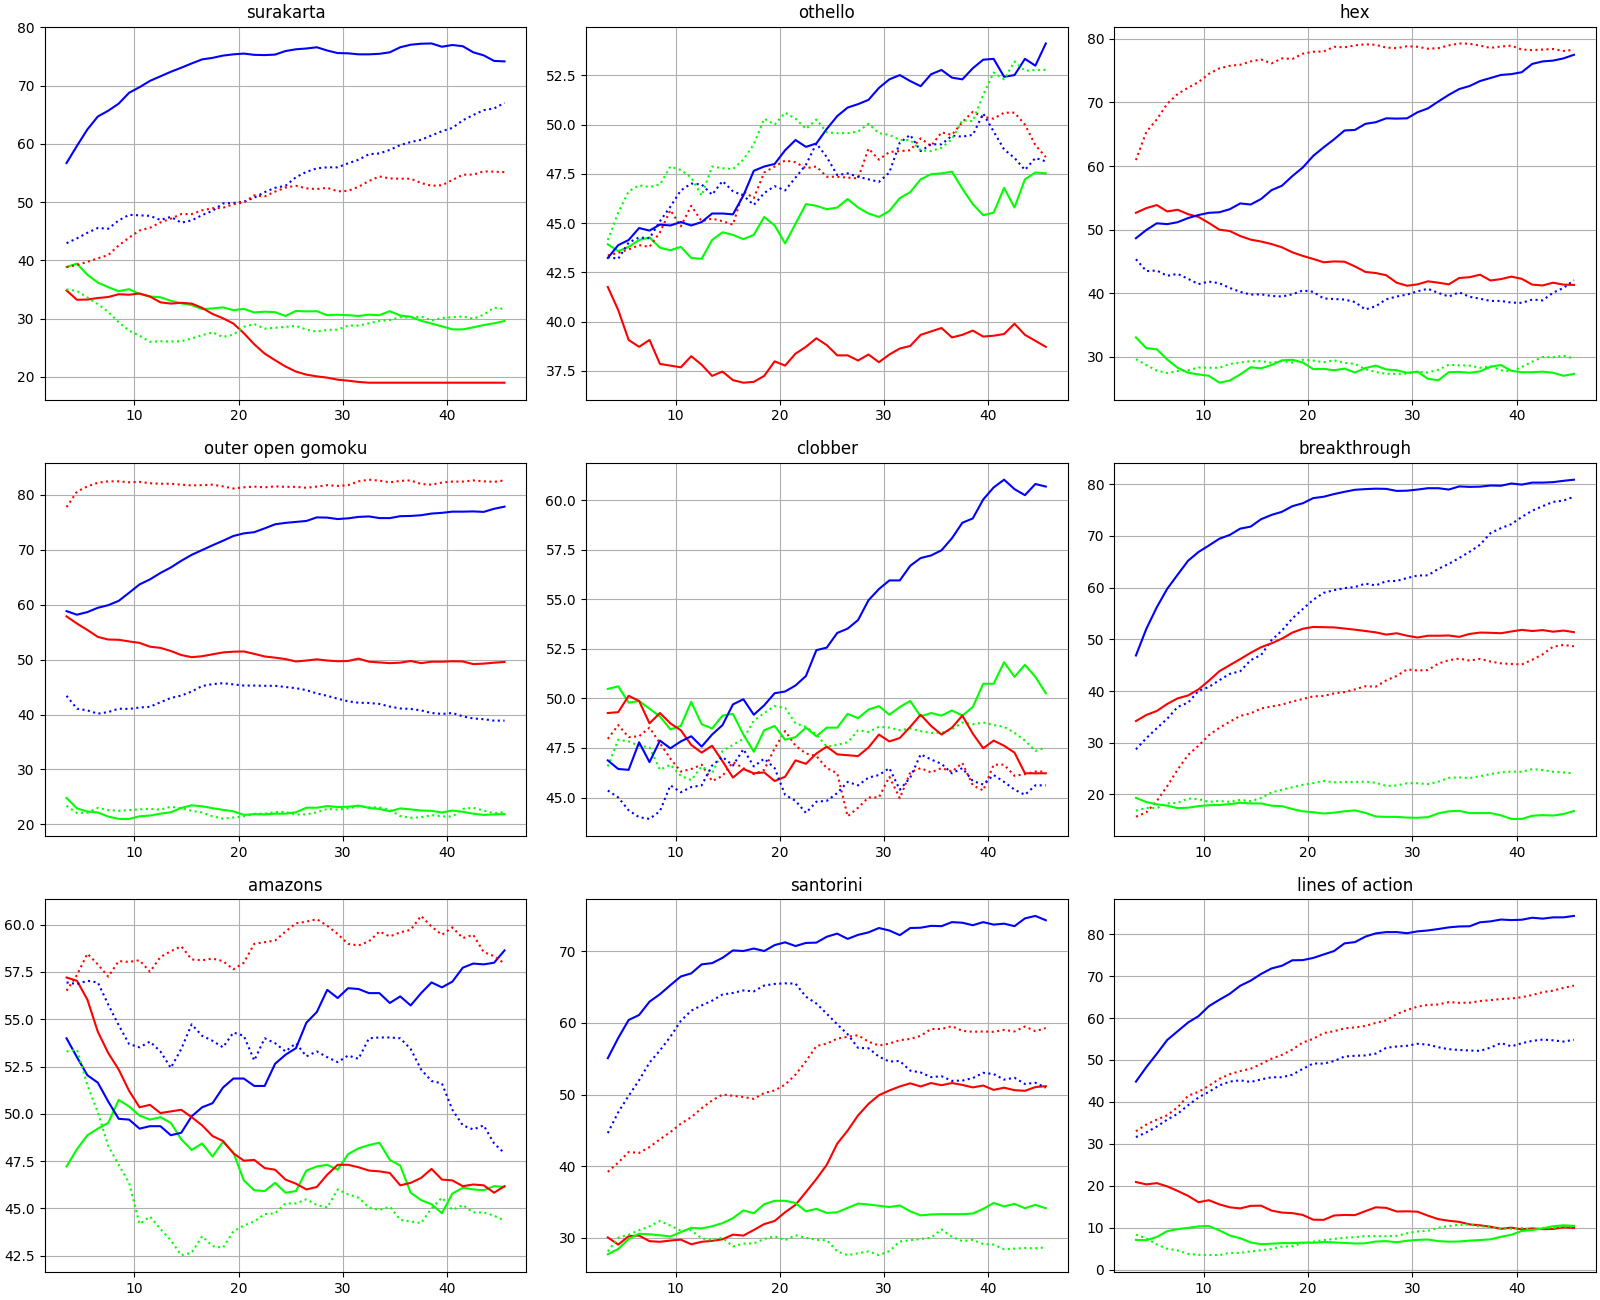
\includegraphics[scale=0.3]{xp0_v2}
\par\end{centering}
\caption{Evolutions of the winning percentages of the combinations of the experiment
of Section~\ref{subsec:Comparison-data-selection}, i.e. MCTS (dotted
line) or iterative deepening alpha-beta (continuous line) with tree
learning (blue line) or root learning (red line) or terminal learning
(green line). The display uses a simple moving average of 6 data.\label{fig:comparison-data}}
\end{figure}
 
\begin{table}
\begin{centering}
\begin{tabular}{|c|c|c|c|c|c|c|}
\hline 
 & \multicolumn{2}{c|}{tree learning} & \multicolumn{2}{c|}{root learning} & \multicolumn{2}{c|}{terminal learning}\tabularnewline
\hline 
 & MCTS & $\id$ & MCTS & $\id$ & MCTS & $\id$\tabularnewline
\hline 
\hline 
Othello & $48.8\%$  & $55.4\%$  & $51.0\%$  & $31.9\%$  & $52.9\%$  & $43.7\%$ \tabularnewline
\hline 
Hex & $45.1\%$  & $79.8\%$  & $79.8\%$  & $44.1\%$  & $29.8\%$  & $27.8\%$ \tabularnewline
\hline 
Clobber & $41.5\%$  & $62.5\%$  & $50.0\%$  & $45.5\%$  & $45.7\%$  & $49.8\%$ \tabularnewline
\hline 
Outer Open Gomoku & $40.3\%$  & $80.0\%$  & $87.3\%$  & $48.8\%$  & $21.6\%$  & $23.1\%$ \tabularnewline
\hline 
Amazons & $46.2\%$  & $58.8\%$  & $56.1\%$  & $44.5\%$  & $39.4\%$  & $46.0\%$ \tabularnewline
\hline 
Breakthrough & $78.1\%$  & $79.2\%$  & $45.5\%$  & $50.6\%$  & $22.3\%$  & $14.3\%$ \tabularnewline
\hline 
Santorini & $50.2\%$  & $73.8\%$  & $60.5\%$  & $51.3\%$  & $29.4\%$  & $36.5\%$ \tabularnewline
\hline 
Surakarta & $69.4\%$  & $65.2\%$  & $56.2\%$  & $20.8\%$  & $28.9\%$  & $23.6\%$ \tabularnewline
\hline 
Lines of Action & $58.8\%$  & $81.7\%$  & $67.7\%$  & $9.6\%$  & $6.9\%$  & $2.7\%$ \tabularnewline
\hline 
\textbf{mean} & $53.1\%$  & $70.7\%$  & $61.6\%$  & $38.5\%$  & $30.8\%$  & $29.7\%$ \tabularnewline
\hline 
\end{tabular}
\par\end{centering}
\caption{Final winning percentages of the combinations of the experiment of
Section~\ref{subsec:Comparison-data-selection} ($\protect\id$:
iterative deepening alpha-beta). Reminder: the percentage is the average
over the repetitions, of the winning percentage of a combination against
each other combination, in first and second player (see~\ref{subsec:Common-Experience-Protocol}
; $95\%$ confidence intervals: max $\pm0.85\%$). \label{tab:comparison-data}}
\end{table}


\section{Tree Search Algorithms for Game Learning\label{sec:Search-Algorithms-for-Learning}}

In this section, we introduce a new tree search algorithm, that we
call \emph{descent minimax} or more succinctly \emph{descent}, dedicated
to be used during the learning process. It requires tree learning
(combining it with root learning or terminal learning is of no interest\footnote{Because, with root and terminal learning, the extra computations of
descent compared to $\ubfm$ with the same number of iterations, do
not change, in general, the values to learn and the move to play (but
the time to perform the iterations is much longer).}). After presenting descent, we compare it to MCTS with root learning
and with tree learning, to iterative deepening alpha-beta with root
learning and with tree learning and to $\ubfm$ with tree learning.

\subsection{Descent: Generate Better Data\label{subsec:Descente-:-g=00003D0000E9n=00003D0000E9rer}}

\begin{algorithm}[!bh]
\DontPrintSemicolon\SetAlgoNoEnd

\SetKwFunction{descenteiteration}{descent\_iteration}

\SetKwFunction{descente}{descent}\SetKwFunction{time}{time}\SetKwFunction{actions}{actions}\SetKwFunction{bestaction}{best\_action}\SetKwFunction{terminal}{terminal}\SetKwFunction{premier}{first\_player}
\SetKwProg{myproc}{Function}{}{}

\myproc{\descenteiteration{$s$, $S$, $T$, $\hadapt$, $\hterminal$}}{

\eIf{\terminal{$s$}}{

$S\leftarrow S\cup\{s\}$\;

$v(s)\leftarrow\hterminal(s)$

}{

\If{$s\notin S$}{

$S\leftarrow S\cup\{s\}$\;

\ForEach{$a\in$ \actions{$s$}}{

\eIf{\terminal{$a(s)$}}{

$S\leftarrow S\cup\{a(s)\}$\;

$v'(s,a)\leftarrow\hterminal\left(a(s)\right)$\;

$v(a(s))\leftarrow v'(s,a)$\;

}{

$v'(s,a)\leftarrow\hadapt\left(a(s)\right)$\;

}

}}

$a_{b}\leftarrow$ \bestaction{$s$}\;

$v'(s,a_{b})\leftarrow$ \descenteiteration{$a_{b}(s)$}\;

$a_{b}\leftarrow$ \bestaction{$s$}\;

$v(s)\leftarrow v'(s,a_{b})$\;

}

return $v(s)$\;

}

\;

\myproc{\bestaction{$s$}}{

\eIf{\premier{$s$}}{return ${\displaystyle \argmax_{a\in\actions{s}}v'\left(s,a\right)}$\;}{return
${\displaystyle \argmin_{a\in\actions{s}}v'\left(s,a\right)}$\;}

}

\;

\myproc{\descente{$s$, $S$, $T$, $\hadapt$, $\hterminal$,
$\tau$}}{

$t=$ \time{}\;

\lWhile{\time{}$-\,t<\tau$}{\descenteiteration{$s$, $S$,
$T$, $\hadapt$, $\hterminal$}}

return $S$, $T$\;

}\;

\protect\protect

\caption{\emph{Descent} tree search algorithm (see Table~\ref{tab:Index-of-symbols}
for the definitions of symbols ; note: $S$ is the set of states which
are non-leaves or terminal and $T=(v,v')$).\label{alg:descente}}
\end{algorithm}

Thus, we present \emph{descent.} It is a modification of $\ubfm$
which builds a different, deeper, game tree, to be combined with tree
learning. The idea of \emph{descent} is to combine $\ubfm$ with deterministic
end-game simulations providing interesting values from the point of
view of learning. The algorithm \emph{descent} (Algorithm~\ref{alg:descente})
recursively selects the best child of the current node, which becomes
the new current node. It adds the children of the current node if
they are not in the tree. It performs this recursion from the root
(the current state of the game) until reaching a terminal node (an
end game). It then updates the value of the selected nodes (minimax
value). The algorithm \emph{descent} repeats this recursive operation
starting from the root as long as there is some search time left.
\emph{Descent} is almost identical to $\ubfm$. The only difference
is that \emph{descent} performs an iteration until reaching a terminal
state while $\ubfm$ performs this iteration until reaching a leaf
of the tree ($\ubfm$ stops the iteration much earlier). In other
words, during an iteration, $\ubfm$ just extends one of the leaves
of the game tree while \emph{descent} recursively extends the best
child from this leaf until reaching the end of the game. The algorithm
\emph{descent} has the advantage of $\ubfm$, i.e. to perform a longer
search to determine a better action to play. By learning the values
of the game tree (by using for example tree learning), it also has
the advantage of a minimax search at depth $1$, i.e. to raise the
values of the terminal nodes to the other nodes more quickly. In addition,
the states thus generated are closer to the terminal states. Their
values are therefore better approximations.
\begin{rem}
In the experiments of this article, when there is a value tie in best\_action(s),
the tie is broken at random. An alternative could be to choose the
subtree whose principal variation is the least deep.
\end{rem}


\subsection{Comparison of Search Algorithms for Game Learning\label{subsec:Comparison-of-algorithms-for-Learning}}

We now compare descent with tree learning to MCTS with root learning
and with tree learning, to iterative deepening alpha-beta with root
learning and with tree learning, and to $\ubfm$ with tree learning,
using the protocol of Section~\ref{subsec:Common-Experience-Protocol}.
Each combination uses one of these tree search algorithms combined
with tree/root learning. There are a total of $6$ combinations. The
experiment was repeated $32$ times. The winning percentage of a
combination for each game and for each evaluation step (i.e. each
hour) is therefore calculated from $192$ matches. The winning percentage
curves are shown in Figure~\ref{fig:comparison-search}. The final
winning percentages are shown in Table~\ref{tab:comparison-search}.
Each percentage of the table has required $6144$ matches. It is descent
which gets the best curves on all games. For two games (Surakarta
and Outer Open Gomoku), the difference with $\ubfm$ is very narrow
but the results remain better than the classic approaches (MCTS and
alpha-beta). On each game, descent obtains a final percentage higher
than all the other combinations (except in Santorini where it is $2\%$
lower than $\ubfm$, the best algorithm at this game). On average
over all games, descent has $82\%$ win and is above $\ubfm$, the
second best combination, by $18\%$ and $\id$ with tree learning,
the third best combination, by $34\%$.
\begin{figure}
\begin{centering}
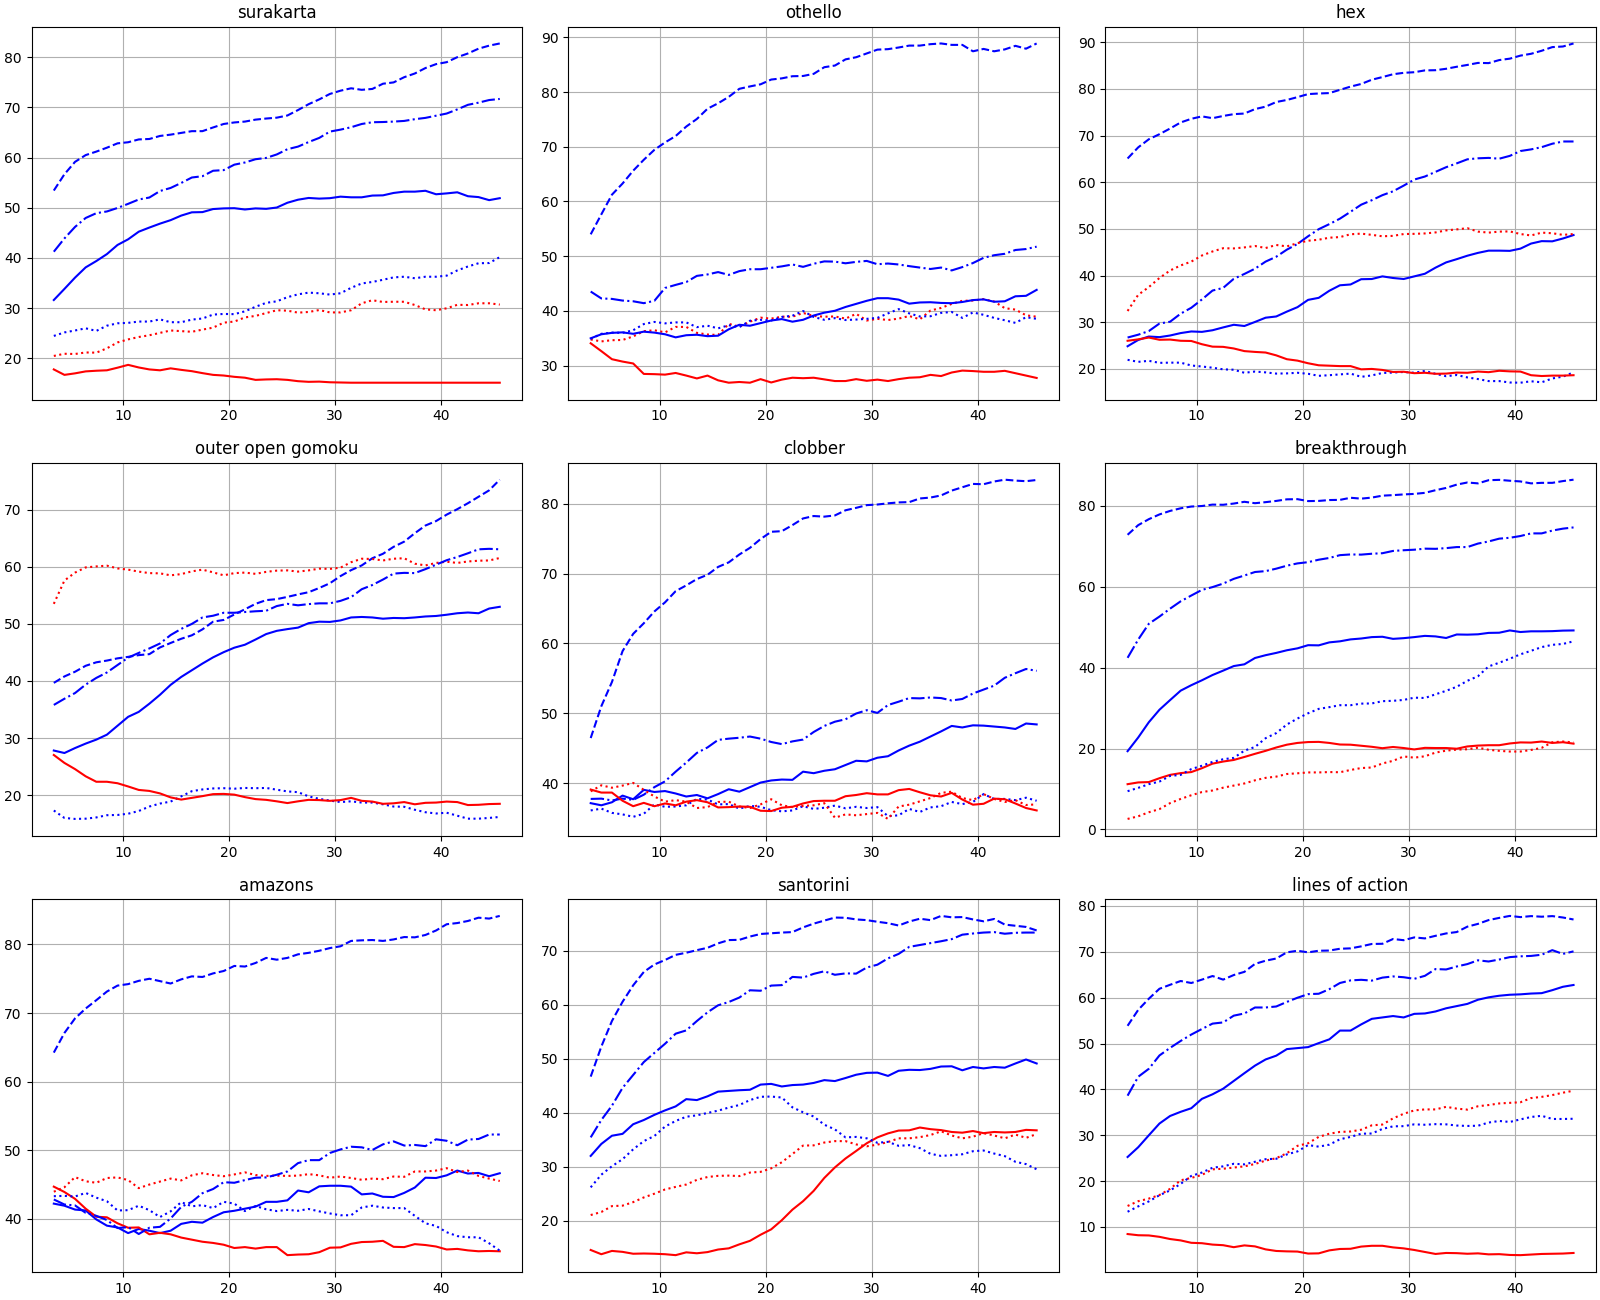
\includegraphics[scale=0.3]{xp1_v2}
\par\end{centering}
\caption{Evolutions of the winning percentages of the combinations of the experiment
of Section~\ref{subsec:Comparison-of-algorithms-for-Learning}, i.e.
of descent (dashed line), $\protect\ubfm$ (dotted dashed line), MCTS
(dotted line), iterative deepening alpha-beta (continuous line) with
tree learning (blue line) or root learning (red line). The display
uses a simple moving average of 6 data.\label{fig:comparison-search}}
\end{figure}
\begin{table}
\begin{centering}
\begin{tabular}{|c|c|c|c|c|c|c|}
\hline 
 & \multicolumn{4}{c|}{tree learning} & \multicolumn{2}{c|}{root learning}\tabularnewline
\hline 
 & descent & $\ubfm$ & MCTS & $\id$ & MCTS & $\id$\tabularnewline
\hline 
\hline 
Othello & $89.4\%$  & $47.2\%$  & $37.7\%$  & $42.7\%$  & $44.9\%$  & $22.1\%$ \tabularnewline
\hline 
Hex & $94.9\%$  & $71.7\%$  & $20.5\%$  & $50.7\%$  & $50.2\%$  & $20.5\%$ \tabularnewline
\hline 
Clobber & $83.0\%$  & $56.7\%$  & $32.9\%$  & $48.9\%$  & $42.0\%$  & $35.5\%$ \tabularnewline
\hline 
Outer Open Gomoku & $77.6\%$  & $63.9\%$  & $18.0\%$  & $51.6\%$  & $64.7\%$  & $18.2\%$ \tabularnewline
\hline 
Amazons & $84.3\%$  & $55.3\%$  & $32.5\%$  & $46.3\%$  & $43.7\%$  & $31.7\%$ \tabularnewline
\hline 
Breakthrough & $86.5\%$  & $72.5\%$  & $45.5\%$  & $47.6\%$  & $19.2\%$  & $21.0\%$ \tabularnewline
\hline 
Santorini & $69.9\%$  & $71.8\%$  & $31.9\%$  & $47.6\%$  & $37.7\%$  & $40.2\%$ \tabularnewline
\hline 
Surakarta & $82.8\%$  & $69.7\%$  & $41.2\%$  & $42.1\%$  & $29.4\%$  & $14.5\%$ \tabularnewline
\hline 
Lines of Action & $73.4\%$  & $66.9\%$  & $36.1\%$  & $57.4\%$  & $39.4\%$  & $3.7\%$ \tabularnewline
\hline 
\textbf{mean} & $82.4\%$  & $64.0\%$  & $32.9\%$  & $48.3\%$  & $41.2\%$  & $23.1\%$ \tabularnewline
\hline 
\end{tabular}
\par\end{centering}
\caption{Final winning percentages of the combinations of the experiment of
Section~\ref{subsec:Comparison-of-algorithms-for-Learning} ($\protect\id$:
iterative deepening alpha-beta ; see~\ref{subsec:Common-Experience-Protocol}
; $95\%$ confidence intervals: max $\pm0.85\%$)\label{tab:comparison-search}}
\end{table}
In conclusion, descent (with tree learning) is undoubtedly the best
combination. $\ubfm$ (with tree learning) is the second best combination,
sometimes very close to descent performances and sometimes very far,
but always superior to other combinations (slightly or largely depending
on the game).

\section{Reinforcement Heuristic to Improve Learning Performance\label{sec:Reinforcement-Heuristic}}

In this section, we propose the technique of \emph{reinforcement heuristic},
which consists to replace the classical terminal evaluation function
-- that we denote by $\hfb$, which returns $1$ if the first player
wins, $-1$ if the second player wins, and $0$ in case of a draw
\citep{young2016neurohex,silver2017mastering,gao2018three} -- by
another heuristic to evaluate terminal states during the learning
process. By using this technique, non-terminal states are therefore
evaluated differently, partial game trees and thus matches during
the learning process are different, which can impact the learning
performances. We start by defining what we call a reinforcement heuristic
and we offering several reinforcement heuristics. Then, we propose
a complementary technique, that we call \emph{completion}, which corrects
state evaluation functions taking into account the resolution of states.
Finally, we compare the reinforcement heuristics that we propose to
the classical terminal evaluation function. 

\subsection{Some Reinforcement Heuristics}

A reinforcement heuristic is a terminal evaluation function that is
more expressive than the classical terminal function, i.e. the game
gain.
\begin{defn}
Let $\hfb$ the game gain function of a game (i.e. $\hfb$ returns
$1$ if the first player wins, $-1$ if the second player wins, and
$0$ in case of a draw). 

A reinforcement heuristic $h_{r}$ is a function that preserves the
order of the game gain function: for any two terminal states of the
game $s,s'$, $\hfb\left(s\right)<\hfb\left(s'\right)$ implies $h_{r}\left(s\right)<h_{r}\left(s'\right)$.
\end{defn}

In the following subsections, we propose different reinforcement heuristics.

\subsubsection{Scoring}

Some games have a natural reinforcement heuristic: the game score.
For example, in the case of the game Othello (and in the case of the
game Surakarta), the game score is the number of its pieces minus
the number of pieces of his opponent (the goal of the game is to have
more pieces than its opponent at the end of the game). The scoring
heuristic used as a reinforcement heuristic consists of evaluating
the terminal states by the final score of the game. With this reinforcement
heuristic, the adaptive evaluation function will seek to learn the
score of states. In the context of an algorithm based on minimax,
the score of a non-terminal state is the minimax value of the subtree
starting from this state whose terminal leaves are evaluated by their
scores. After training, the adaptive evaluation function then contains
more information than just an approximation of the result of the game,
it contains an approximation of the score of the game. If the game
score is \emph{intuitive}, this should improve learning performances. 
\begin{rem}
In the context of the game of the Amazons, the score is the size of
the territory of the winning player, i.e. the squares which can be
reached by a piece of the winning player. This is approximately the
number of empty squares.
\end{rem}


\subsubsection{Additive and Multiplicative Depth Heuristics\label{subsec:Depth-Heuristic}}

Now we offer the following reinforcement heuristic: the \emph{depth
heuristic}. It consists in giving a better value to the winning states
close to the start of the game than to the winning states far from
the start. Reinforcement learning with the depth heuristic, it is
learning the duration of matches in addition to their results. This
learned information is then used to try to win as quickly as possible
and try to lose as late as possible. The hypothesis of this heuristic
is that a state close to the end of the game has a more precise value
than a state more distant and that the duration of the game is easily
learned. Under this assumption, with this heuristic, we will take
less risk to try to win as quickly as possible and to lose as late
as possible. In addition, with a long game, a player in difficulty
will have more opportunities to regain the upper hand. We propose
two realizations of the depth heuristic: the \emph{additive depth
heuristic}, that we denote by $\hfp$, and the\emph{ multiplicative
depth heuristic}, that we denote by $\hfp'$. The evaluation function
$\hfp$ returns the value $l$ if the first player wins, the value
$-l$ if the second player wins, and $0$ in case of a draw, with
$l=P-p+1$ where $P$ is the maximum number of playable actions in
a game and $p$ is the number of actions played since the beginning
of the game. For the game of Hex, $l$ is the number of empty cells
on the board plus $1$. For the games where $P$ is very large or
difficult to compute, we can instead use $l=\max\left(1,\tilde{P}-p\right)$
with $\tilde{P}$ a constant approximating $P$ (close to the empirical
average length of matches).The evaluation function $\hfp'$ is identical
except that $l$ satisfies $l=\frac{\tilde{P}}{p}$.
\begin{rem}
Note that the idea of fast victory and slow defeat has already been
proposed but not used in a learning process~\citep{CazenaveSST16}.
\end{rem}


\subsubsection{Cummulative Mobility\label{subsec:Cummulative-Mobility}}

The next reinforcement heuristic that we propose is \emph{cummulative
mobility}. It consists in favoring the games where the player has
more possibility of action and where his opponent has less. The implementation
used in this article is as following. The value of a terminal state
is $\frac{M_{1}}{M_{2}}$ if the first player wins, $-\frac{M_{2}}{M_{1}}$
if the second player wins, and $0$ in case of a draw, where $M_{1}$
is the mean of the number of available actions in each turn of the
first player since the start of the game and $M_{2}$ is the mean
of the number of available actions in each turn of the second player
since the start of the game.

\subsubsection{Piece Counting: Presence}

Finally, we propose as reinforcement heuristic: the \emph{presence}
heuristic. It consists in taking into account the number of pieces
of each player and starts from the assumption that the more a player
has pieces the more this one has an advantage. There are several implementations
for this heuristic, we use in this article the following implementation:
the heuristic value is $\max(n_{1}-n_{2},1)$ if the first player
wins, $\min(n_{1}-n_{2},-1)$ if the second player wins, and $0$
in case of a draw, where $n_{1}$ is the number of pieces of the first
player and $n_{2}$ is the number of pieces of the second player.
Note that in the games Surakarta and Othello, the score corresponds
to a presence heuristic.

\subsection{Completion\label{subsec:Completion}}

Relying solely on the value of states calculated from the terminal
evaluation function \emph{and} the adaptive evaluation function can
sometimes lead to certain aberrant behaviors. More precisely, if we
only seek to maximize the value of states, we will then choose to
play a state $s$ rather than another state $s'$ if $s$ is of greater
value than $s'$ even if $s'$ is a winning resolved state (a state
is \emph{resolved} if we know the result of the game starting from
this state in which the two players play optimally). A search algorithm
can resolve a state. This happens when all the leaves of the subtree
starting from this state are terminal. Choosing $s$ rather than $s'$,
a winning resolved state, is an error\footnote{There is perhaps, in certain circumstances, an interest in making
this error from the point of view of learning.} when $s$ is not resolved (or when $s$ is resolved and is not winning).
By choosing $s$, guarantee of winning is lost. The left graph of
Figure~\ref{fig:completion} illustrates such a scenario. 
\begin{figure}
\begin{centering}
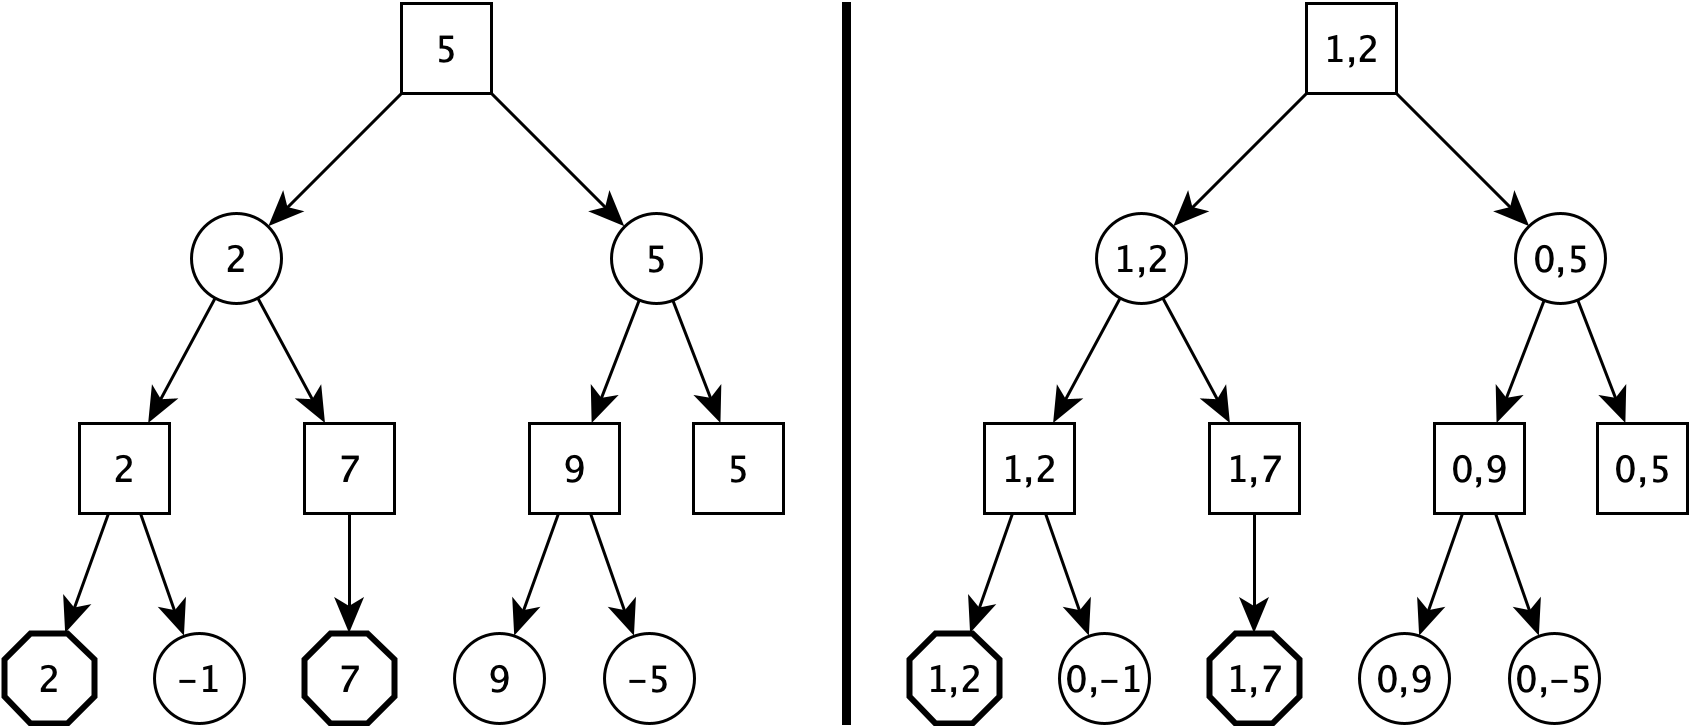
\includegraphics[scale=0.28]{completed_non_completed_tree}
\par\end{centering}
\caption{The left graph is a game tree where maximizing does not lead to the
best decision ; the right graph is the left game tree with completion
(nodes are labeled by a pair of values) and thus maximizing leads
to the best decision (square node: first player node (max node), circle
node: second player node (min node), octagon: terminal node)\label{fig:completion}. }
\end{figure}
It is therefore necessary to take into account both the value of states
and the resolution of states. The completion technique, which we propose
in this section, is one way of doing it. It consists, on the one hand,
in associating with each state $s$ a completion value $c(s)$ and
a resolution value $r(s)$. The completion value $c(s)$ of a leaf
state $s$ is $0$ if the state $s$ is not terminal or if it is
a draw, $1$ if it is a winning terminal state and $-1$ if the state
is a losing terminal state. The value $c(s)$ of a non-leaf state
$s$ is computed as the minimax value of the subtree of the partial
game tree starting from $s$ where the leaves are evaluated by their
completion value. The resolution value $r(s)$ of a leaf state $s$
is $0$ if the state $s$ is not terminal and $1$ if it is terminal.
The resolution value $r(s)$ of a non-leaf state $s$ is $1$ if
$\left|c\left(s\right)\right|=1$. Otherwise, $r(s)$ is the minimum
of the resolution values of the childen of $s$. The completion technique
consists, on the other hand, in using $c\left(\cdot\right)$ to compute
$v\left(\cdot\right)$. For this, states are compared from pairs $\left(c\left(\cdot\right),v\left(\cdot\right)\right)$,
by using the lexicographic order (instead of just compare states from
$v\left(\cdot\right)$). More precisely, the value $v\left(s\right)$
of a state $s$ is computed in calculating $\left(c(s),v(s)\right)$
as the minimax value of the subtree of the partial game tree starting
from $s$ where the leaves $l$ are evaluated by $\left(c(l),v(l)\right)$.
Thus, the value $v\left(s\right)$ of a winning state $s$ is always
the value of the corresponding winning terminal leaf. Finally, with
the completion technique, to decide which action to play during the
search, we choose the best unresolved action if it exists and otherwise
the best resolved action (i.e. we choose the action which maximize
$\left(-r\left(s\right),c\left(s\right),v\left(s\right)\right)$ in
a max state and which minimize $\left(r\left(s\right),c\left(s\right),v\left(s\right)\right)$
in a min state). The right graph of Figure~\ref{fig:completion}
illustrates the use of completion. The use of the resolution of states
also makes it possible to stop the search in the resolved subtrees
and thus to save computing time. Descent algorithm modified to use
the completion and the resolution stop is described in Algorithm~\ref{alg:descente-completion}.
With completion, descent always chooses an action leading to a winning
resolved state and never chooses, if possible, an action leading to
a losing resolved state.
\begin{rem}
For a game where there is no draw, the computation of the resolution
value is not necessary (all necessary information is in the completion
value).
\end{rem}

\begin{rem}
A variant consists in performing a strong resolution, i.e. to compute
$r\left(\cdot\right)$ for non-leaf states in the following way: $r\left(s\right)$
is (in all cases) the minimum of the resolution values of the childen
of the state $s$. With this variant, unnecessary calculations are
made to determine the best action to play. However, the additional
values may be useful for learning. It is not clear which variant is
the best.

Another variant is possible, it consists in not using the completition
$c\left(\cdot\right)$ to compute $v\left(\cdot\right)$. With this
version, $v\left(s\right)$ is the minimax value of the subtree starting
from $s$ where the leaf nodes $l$ are evaluated by $v\left(l\right)$.
With this variant, for certain resolved states, instead of learning
a lower bound (in absolute value), which is an exact value, we learn
an estimated value, which could be a potentially an overestimated
value. It is not clear which variant is the best.
\end{rem}

\begin{algorithm}[!bh]
\DontPrintSemicolon\SetAlgoNoEnd

\SetKwFunction{completiondescenteiteration}{completed\_descent\_iteration}

\SetKwFunction{completiondescente}{completed\_descent}\SetKwFunction{time}{time}\SetKwFunction{actions}{actions}\SetKwFunction{completedbestaction}{completed\_best\_action}\SetKwFunction{completedbestactiondual}{completed\_best\_action\_dual}\SetKwFunction{terminal}{terminal}\SetKwFunction{premier}{first\_player}
\SetKwFunction{backupresolution}{backup\_resolution} \SetKwProg{myproc}{Function}{}{}

\myproc{\completiondescenteiteration{$s$, $S$, $T$, $\hadapt$,
$\hterminal$}}{

\eIf{\terminal{$s$}}{

$S\leftarrow S\cup\{s\}$\;

$r\left(s\right),c\left(s\right),v\left(s\right)\leftarrow1,\hfb(s),\hterminal(s)$

}{

\If{$s\notin S$}{

$S\leftarrow S\cup\{s\}$\;

\ForEach{$a\in$ \actions{$s$}}{

\eIf{\terminal{$a(s)$}}{

$S\leftarrow S\cup\{a(s)\}$\;

$v'(s,a)\leftarrow\hterminal\left(a(s)\right)$\;

$r(a(s)),c(a(s)),v(a(s))\leftarrow1,\hfb(a(s)),v'(s,a)$\;

}{

$v'(s,a)\leftarrow\hadapt\left(a(s)\right)$\;

}

}

$a_{b}\leftarrow$ \completedbestaction{$s$, $\actions{s}$}\;

$c(s),v(s)\leftarrow c\left(a_{b}(s)\right),v'\left(s,a_{b}\right)$\;

$r\left(s\right)\leftarrow$ \backupresolution{$s$}\;

}

\If{$r\left(s\right)=0$}{

$A\leftarrow\liste{a\in\actions{s}}{r\left(a\left(s\right)\right)=0}$

$a_{b}\leftarrow$ \completedbestactiondual{$s$, $A$}\;

$n(s,a_{b})\leftarrow n(s,a_{b})+1$\;

$v'\left(s,a_{b}\right)\leftarrow$ \completiondescenteiteration{$a_{b}(s)$}\;

$a_{b}\leftarrow$ \completedbestaction{$s$, $\actions{s}$}\;

$c(s),v(s)\leftarrow c\left(a_{b}(s)\right),v'\left(s,a_{b}\right)$\;

$r\left(s\right)\leftarrow$ \backupresolution{$s$}\;

}

}

return $v\left(s\right)$\;

}

\;

\myproc{\completiondescente{$s$, $S$, $T$, $\hadapt$, $\hterminal$,
$\tau$}}{

$t=$ \time{}\;

\lWhile{\time{}$-\,t<\tau$ $\wedge$ $r\left(s\right)=0$}{\completiondescenteiteration{$s$,
$S$, $T$, $\hadapt$, $\hterminal$}}

return $S$, $T$\;

}\;

\protect\protect

\caption{\emph{Descent} tree search algorithm with completion and resolution
stop (see Table~\ref{tab:Index-of-symbols} for the definitions of
symbols and Algorithm~\ref{alg:descente-completion-suite} for the
definitions of completed\_best\_action($s$) and backup\_resolution($s$)).
Note: $T=(v,v',c,r)$ and $S$ is the set of states of the partial
game tree which are non-leaves or terminal.\label{alg:descente-completion}}
\end{algorithm}
\begin{algorithm}[!bh]
\DontPrintSemicolon\SetAlgoNoEnd

\SetKwFunction{completiondescenteiteration}{completed\_descent\_iteration}

\SetKwFunction{completiondescente}{completed\_descent}\SetKwFunction{time}{time}\SetKwFunction{actions}{actions}\SetKwFunction{completedbestaction}{completed\_best\_action}\SetKwFunction{completedbestactiondual}{completed\_best\_action\_dual}\SetKwFunction{terminal}{terminal}\SetKwFunction{premier}{first\_player}
\SetKwFunction{backupresolution}{backup\_resolution} \SetKwProg{myproc}{Function}{}{}

\myproc{\completedbestaction{$s$, $A$}}{

\eIf{\premier{$s$}}{return ${\displaystyle \argmax_{a\in A}\left(c\left(a\left(s\right)\right),v'\left(s,a\right),n\left(s,s'\right)\right)}$\;}{return
${\displaystyle \argmin_{a\in A}\left(c\left(a\left(s\right)\right),v'\left(s,a\right),-n\left(s,s'\right)\right)}$\;}

}

\;

\myproc{\completedbestactiondual{$s$, $A$}}{

\eIf{\premier{$s$}}{return ${\displaystyle \argmax_{a\in A}\left(c\left(a\left(s\right)\right),v'\left(s,a\right),-n\left(s,s'\right)\right)}$\;}{return
${\displaystyle \argmin_{a\in A}\left(c\left(a\left(s\right)\right),v'\left(s,a\right),n\left(s,s'\right)\right)}$\;}

}

\;

\myproc{\backupresolution{$s$}}{

\eIf{$\left|c\left(s\right)\right|=1$}{return $1$ \;}{return
$\minimum{}_{a\in\actions{s}}r\left(a\left(s\right)\right)$\;}

}

\;

\protect\protect

\caption{Definition of the algorithms completed\_best\_action($s$, $A$),
which computes the \emph{a priori }best action by using completion,
and backup\_resolution($s$), which updates the resolution of $s$
from its child states. \label{alg:descente-completion-suite}}
\end{algorithm}

We also propose to use the resolution of states with action selections,
to reduce the duration of games and therefore \emph{a priori} the
duration of the learning process: always play an action leading to
a winning resolved state if it exists and never play an action leading
to a losing resolved state if possible. Thus, if among the available
actions we know that one of the actions is winning, we play it. If
there is none, we play according to the chosen action selection method
among the actions not leading to a resolved state (if possible). If
it is not possible, we play the best action leading to a state resolved
as a draw and if there is none, we play the best action leading to
a losing resolved state. We call it \emph{completed action selection}.
\begin{rem}
It is not clear, however, that this improves performance as it prunes
a portion of the game tree in the exploration whose values could be
useful for learning (but could also negatively impact the learning
performance).
\end{rem}


\subsection{Comparison of Reinforcement Heuristics\label{subsec:Comparison-of-Reinforcement}}

We now compare the different heuristics that we have proposed to the
classical terminal evaluation function $\hfb$ on different games,
using the protocol of Section~\ref{subsec:Common-Experience-Protocol}.
Each combination uses descent with completion (Algorithm~\ref{alg:descente-completion})
and completed $\epsilon$-greedy (see Algorithm~\ref{alg:e-greedy}
and Section~\ref{subsec:Completion}). Each combination uses a different
terminal evaluation function. These terminal evaluations are the classical
(``binary'') evaluation function $\hfb$, the additive depth heuristic,
the multiplicative depth heuristic, the scoring heuristic, the cummulative
mobility, and the presence heuristic. Other parameters are the same
as Section~\ref{subsec:Comparison-data-selection}. There are, at
most, a total of $6$ combinations per game (on some games, some
heuristics are not evaluated because they are trivially of no interest
or equivalent to another heuristic). The experiment was repeated $48$
times. The winning percentage of a combination for each game and
for each evaluation step (i.e. each hour) is therefore calculated
from $96$ to $192$ matches. The final winning percentages are shown
in Table~\ref{tab:comparison-h}. Each percentage of the table has
required between $4608$ and $9216$ matches. On average and in $7$
of the $9$ games, the classic terminal heuristic has the worst percentage
(exception are Othello and Lines of Action). In scoring games, scoring
is the best heuristic, as we might expect. Leaving aside the score
heuristic, with the exception of Surakarta, Othello and Clobber, it
is one of the two depth heuristics that has the best winning percentage.
In Surakarta and Clobber, mobility is just ahead of the depth heuristics.
On average, using the additive depth heuristic instead of using the
classic evaluation increases the winning percentage by $15\%$, and
using the best depth heuristic increases the winning percentage by
$19\%$. The winning percentage curves are shown in Figure~\ref{fig:comparison-h}.
The final percentages summarize the curves quite well. Note however,
on the one hand, that the clear impact compared to the other heuristics
(except score) of the additive depth heuristic to Breakthrough, Amazons,
Hex, and Santorini and of the multiplicative depth heuristic to Clobber,
Hex, and Open Outer Gomoku. In conclusion, the use of generic reinforcement
heuristics has significantly improved performances and the depth heuristics
are prime candidates as a powerful generic reinforcement heuristic.
\begin{figure}
\begin{centering}
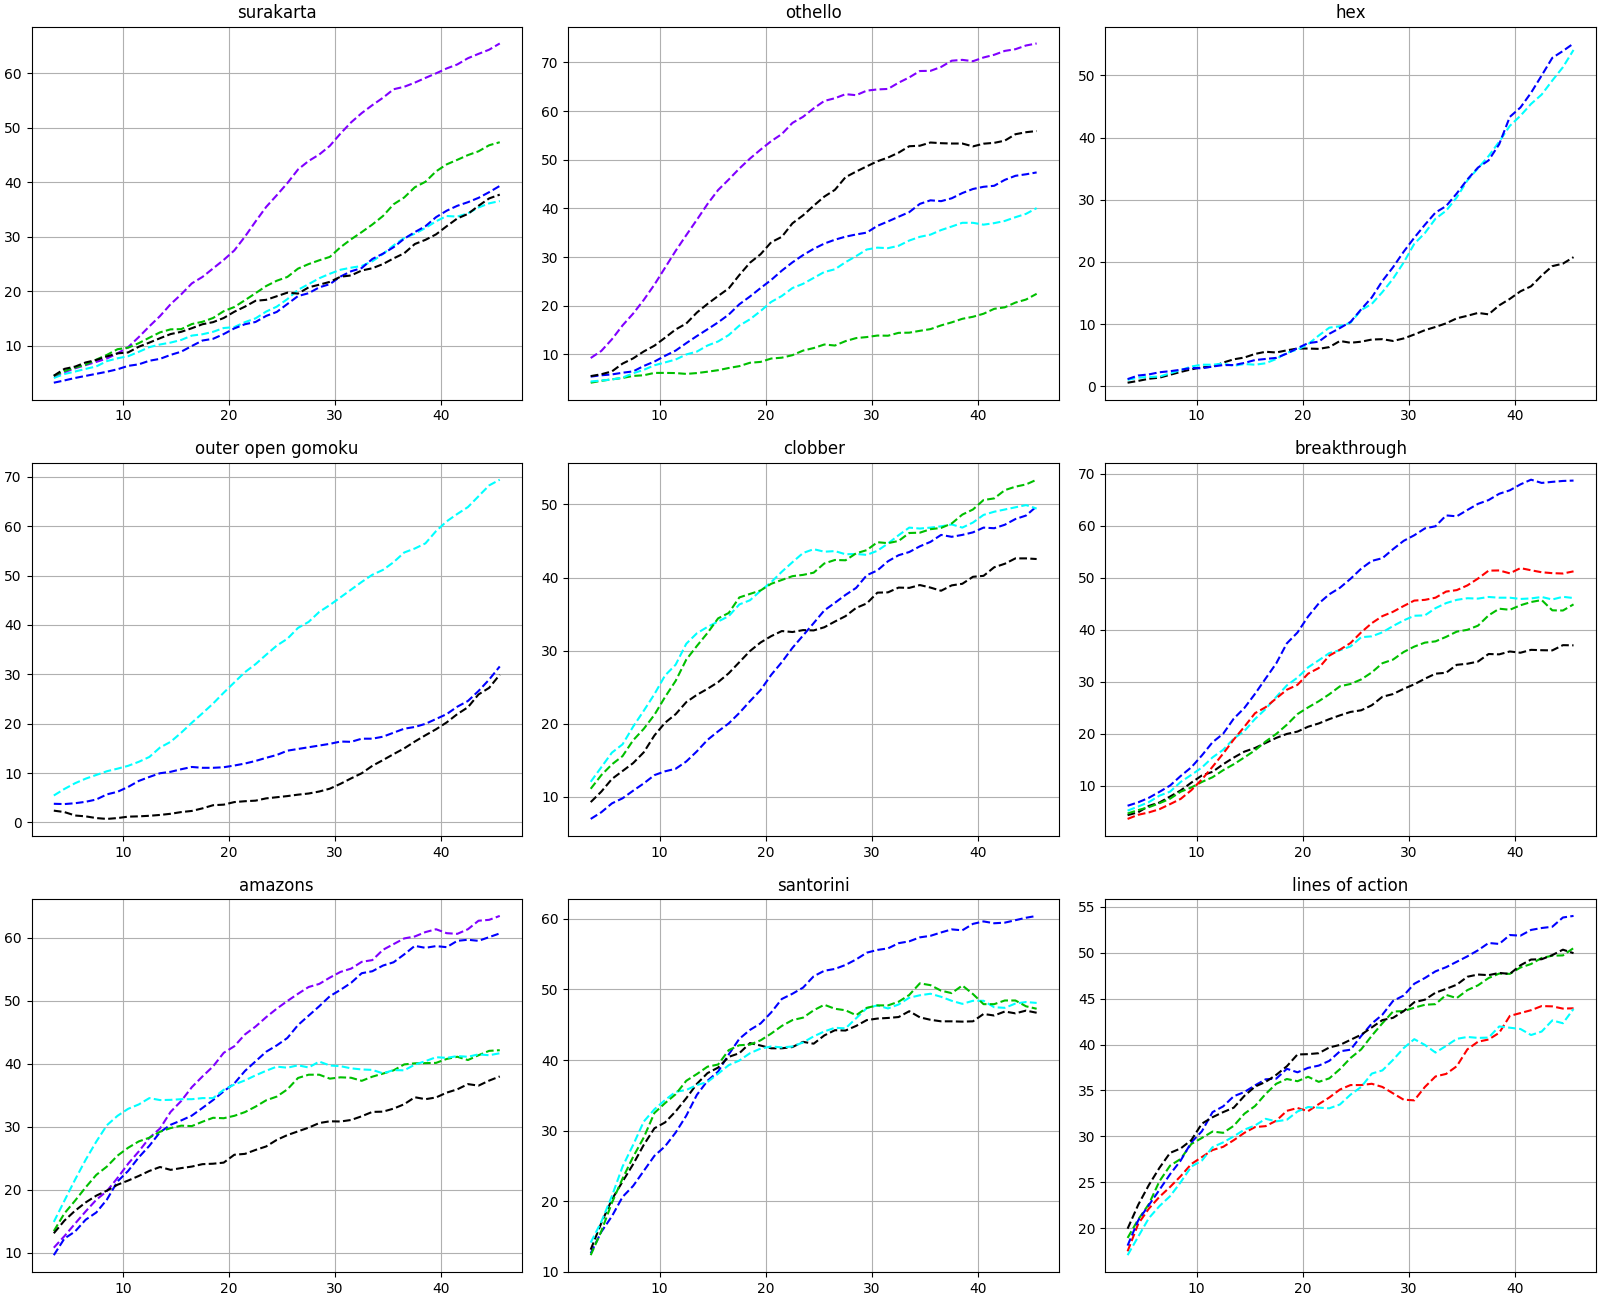
\includegraphics[scale=0.3]{xp_2_v2}
\par\end{centering}
\caption{Evolutions of the winning percentages of the combinations of the experiment
of Section~\ref{subsec:Comparison-of-Reinforcement}, i.e. the use
of the following heuristics: classic (black line), score (purple line),
additive depth (blue line), multiplicative depth (turquoise line),
cumulative mobility (green line), and presence (red line). The display
uses a simple moving average of 6 data.\label{fig:comparison-h}}
\end{figure}
\begin{table}
\begin{centering}
\begin{tabular}{|c|c|c|c|c|c|c|}
\hline 
 &  &  & \multicolumn{2}{c|}{depth} &  & \tabularnewline
\hline 
 & classic & score & additive  & multiplicative  & mobility & presence\tabularnewline
\hline 
\hline 
Othello & $49.8\%$  & $70.6\%$  & $50.1\%$  & $48.9\%$  & $18.5\%$  & score\tabularnewline
\hline 
Hex & $33.3\%$  & X & $66.1\%$  & $60.4\%$  & X & X\tabularnewline
\hline 
Clobber  & $43.7\%$  & X & $47.0\%$  & $49.8\%$  & $53.5\%$  & X\tabularnewline
\hline 
Outer Open Gomoku & $33.0\%$  & X & $41.4\%$  & $74.4\%$  & X & X\tabularnewline
\hline 
Amazons & $36.8\%$  & $67.9\%$  & $60.0\%$  & $50.7\%$  & $49.0\%$  & X\tabularnewline
\hline 
Breakthrough & $39.0\%$  & X & $69.5\%$  & $40.4\%$  & $43.9\%$  & $48.5\%$ \tabularnewline
\hline 
Santorini & $42.7\%$  & X & $59.7\%$  & $46.6\%$  & $43.3\%$  & X\tabularnewline
\hline 
Surakarta & $33.5\%$  & $68.9\%$  & $43.1\%$  & $35.3\%$  & $55.6\%$  & score\tabularnewline
\hline 
Lines of Action & $50.9\%$  & X & $57.1\%$  & $46.8\%$  & $53.7\%$  & $44.0\%$ \tabularnewline
\hline 
\textbf{mean} & $40.3\%$  & $69.1\%$  & $54.9\%$  & $50.4\%$  & $45.4\%$  & $46.3\%$ \tabularnewline
\hline 
\end{tabular}
\par\end{centering}
\caption{Final winning percentages of the combinations of the experiment of
Section~\ref{subsec:Comparison-of-Reinforcement} (X: heuristic without
interest in this context ; presence coincides with score in Surakarta
and Othello ; see~\ref{subsec:Common-Experience-Protocol} ; $95\%$
confidence intervals: max $\pm1.04\%$)\label{tab:comparison-h}}

\end{table}


\section{Search Algorithms for Game Playing\label{sec:Search-Algorithms-for-Playing}}

In this section, we propose another variant of $\ubfm$, dedicated
to be used in competition mode. Then, we compare it with other tree
search algorithms.

\subsection{Unbound Best-First Minimax with Safe Decision: $\protect\ubfmt$}

Thus, we propose a modification of $\ubfm$, denoted $\ubfmt$. It
aims to provide a safer game. The action $\ubfm$ chooses to play
is the one that leads to the state of best value. In some cases, the
(\emph{a priori}) best action can lead to a state that has not been
sufficiently visited (such as a non-terminal leaf). Choosing this
action is therefore a risky decision. We propose, to avoid this problem,
a different decision that aims to play the safest action, in the same
way as MCTS (max child selection \citep{browne2012survey}). If no
action leads to a winning resolved state, the action chosen by $\ubfmt$
is the one that has been the most selected (since the current state
of the game) during the exploration of the game tree. In case of a
tie, $\ubfmt$ decides by choosing the one that leads to the state
of best value. This decision is safer because the number of times
an action is selected is the number of times that this action is more
interesting than the others.
\begin{example}
The current player has the choice between two actions $a_{1}$ and
$a_{2}$. The action $a_{1}$ leads to a state of value $5$ and was
selected $7$ times (from the current state and from the beginning
of the game). The action $a_{2}$ leads to a state of value $2$ and
was selected $30$ times. $\ubfm$ chooses the action $a_{1}$ while
$\ubfmt$ chooses the action $a_{2}$.
\end{example}

The algorithm of $\ubfmt$ with completion is described in Algorithm~\ref{alg:ubfms-decision}
(which uses Algorithm~\ref{alg:ubfms_search} ; resolution stop is
not used for the succinctness of the presentation).

\begin{algorithm}[!bh]
\DontPrintSemicolon\SetAlgoNoEnd

\SetKwFunction{completionubfmsiteration}{ubfms\_iteration}

\SetKwFunction{completionubfms}{ubfms\_tree\_search}\SetKwFunction{time}{time}\SetKwFunction{actions}{actions}\SetKwFunction{completedbestaction}{completed\_best\_action}\SetKwFunction{terminal}{terminal}\SetKwFunction{premier}{first\_player}
\SetKwProg{myproc}{Function}{}{}

\myproc{\completionubfmsiteration{$s$, $S$, $T$, $\hadapt$,
$\hterminal$}}{

\eIf{\terminal{$s$}}{

$S\leftarrow S\cup\{s\}$\;

$r(s),c(s),v(s)\leftarrow1,\hfb(s),\hterminal(s)$

}{

\If{$r\left(s\right)=0$}{

\eIf{$s\notin S$}{

$S\leftarrow S\cup\{s\}$\;

\ForEach{$a\in$ \actions{$s$}}{

\eIf{\terminal{$a(s)$}}{

$S\leftarrow S\cup\{a(s)\}$\;

$v'(s,a)\leftarrow\hterminal\left(a(s)\right)$\;

$r(a(s)),c(a(s)),v(a(s))\leftarrow1,\hfb(a(s)),v'(s,a)$\;

}{

$v'(s,a)\leftarrow\hadapt\left(a(s)\right)$\;

}

}

}{

$A\leftarrow\liste{a\in\actions{s}}{r\left(a\left(s\right)\right)=0}$

$a_{b}\leftarrow$ \completedbestactiondual{$s$, $A$}\;

$n(s,a_{b})\leftarrow n(s,a_{b})+1$\;

$v'\left(s,a_{b}\right)\leftarrow$ \completionubfmsiteration{$a_{b}(s)$}}\;

$a_{b}\leftarrow$ \completedbestaction{$s$, $\actions{s}$}\;

$c(s),v(s)\leftarrow c\left(a_{b}(s)\right),v'\left(s,a_{b}\right)$\;

$r\left(s\right)\leftarrow$ \backupresolution{$s$}\;

}

}

return $v(s)$\;

}

\;

\myproc{\completionubfms{$s$, $S$, $T$, $\hadapt$, $\hterminal$,
$\tau$}}{

$t=$ \time{}\;

\lWhile{\time{}$-\,t<\tau\wedge r\left(s\right)=0$}{\completionubfmsiteration{$s$,
$S$, $T$, $\hadapt$, $\hterminal$}}

return $S$, $T$\;

}\;

\protect\protect

\caption{\emph{$\protect\ubfmt$} tree search algorithm with completion and
resolution stop (see Table~\ref{tab:Index-of-symbols} for the definitions
of symbols and Algorithm~\ref{alg:descente-completion-suite} for
the definitions of completed\_best\_action($s$) and backup\_resolution($s$)).
Note: $T=(v,v',c,r,n)$.\label{alg:ubfms_search}}
\end{algorithm}
\begin{algorithm}[!bh]
\DontPrintSemicolon\SetAlgoNoEnd

\SetKwFunction{completionubfmsiteration}{ubfms\_iteration}

\SetKwFunction{completiontreeubfms}{ubfms\_tree\_search}\SetKwFunction{completionubfms}{ubfms}\SetKwFunction{time}{time}\SetKwFunction{actions}{actions}\SetKwFunction{completedsafestaction}{safest\_action}\SetKwFunction{terminal}{terminal}\SetKwFunction{premier}{first\_player}
\SetKwProg{myproc}{Function}{}{}

\myproc{\completedsafestaction{$s$, $T$}}{

\eIf{\premier{$s$}}{return ${\displaystyle \argmax_{a\in\actions{s}}\left(c(a(s)),n(s,a),v'\left(s,a\right)\right)}$\;}{return
${\displaystyle \argmin_{a\in\actions{s}}\left(c(a(s)),-n(s,a),v'\left(s,a\right)\right)}$\;}

}

\;

\myproc{\completionubfms{$s$, $S$, $T$, $\hadapt$, $\hterminal$,
$\tau$}}{

$S,T\leftarrow$\completiontreeubfms{$s$, $S$, $T$, $\hadapt$,
$\hterminal$}\;

return \completedsafestaction{$s$, $T$}

}\;

\protect\protect

\caption{\emph{$\protect\ubfmt$} action decision algorithm with completion
(see Table~\ref{tab:Index-of-symbols} for the definitions of symbols).
Note: $T=(v,v',c,r,n)$ and $S$ is the set of states of the game
tree which are non-leaves or terminal.\label{alg:ubfms-decision}}
\end{algorithm}

\begin{rem}
In some cases, we will prefer to ensure the draw rather than trying
to win. Algorithm~\ref{alg:ubfms-decision} must then be adapted:
to decide the action to play, the first player must then maximize
$\left(c(a(s)),r\left(a(s)\right),n(s,a),v'\left(s,a\right)\right)$
and the second player must minimize $\left(c(a(s)),-r\left(a(s)\right),n(s,a),v'\left(s,a\right)\right)$.
\end{rem}


\subsection{Comparison of Search Algorithms for Game Playing\label{subsec:Comparison-of-Search}}

We now compare the winning percentages of different game algorithms,
by using evaluation functions learned by starting again the experiment
of Section~\ref{subsec:Comparison-of-algorithms-for-Learning} with
$16$ as repetition number (the used evaluations are those corresponding
to the end of the learning process, i.e. $h=48$). We compare $\ubfmt$
with $\ubfm$ and iterative deepening alpha-beta with move ordering,
denoted $\id$ (each of these algorithms uses completion). For each
game, each combination $(A,\hadaptnum{48},r)$ confronts the combinations
$(A',\hadaptnum{48},r)$, with a search time of $1s$ per action,
where $A\in\left\{ \ubfmt,\ubfm,\id\right\} $, $A'$ is minimax at
depth $1$, $\hadaptnum{48}$ is one of the final evaluation functions
of Section~\ref{subsec:Comparison-of-algorithms-for-Learning}, and
$r$ is the number of one of the $16$ repetitions ($r\in\{1,\ldots,16\}$).
The winning percentage of $A$ is the average of the winning percentage
of $(A,\hadaptnum{48},r)$ over the functions $\hadaptnum{48}$ and
over the repetitions $r\in\{1,\ldots,16\}$. The winning percentages
are described in Table~\ref{tab:competition-percentage-1}. For each
game, the winning percentage of a search algorithm is calculated from
$18432$ matches. On all games except Clobber, $\ubfmt$ gets the
best winning percentage (on two games, Hex and Outer Open Gomoku,
$\ubfmt$ and $\id$ have the same percentage). On Clobber, it is
$\ubfm$ which obtains the best percentage, but only $1\%$ more than
$\ubfmt$ . On average, across all games, $\ubfmt$ is $3.6\%$ better
than $\ubfm$ and $5\%$ better than $\id$.

Then a variation of this experiment was performed. For each game,
each combination $(A,\hadaptnum{48},r)$ confronts all the others,
but the used evaluation functions $\hadaptnum{48}$ are restricted
to those generated from the learning algorithm descent and the search
time is $10s$ per action. The corresponding winning percentages are
described in Table~\ref{tab:competition-percentage-10}. For each
game, the winning percentage of a search algorithm is calculated from
$1536$ matches. In all games, except Clobber and Santorini, it is
again $\ubfmt$ which obtains the best winning percentage. At Clobber
and Santorini, it is $\ubfm$ which obtains the best percentage. On
average across all games, $\ubfmt$ is $5\%$ better than $\ubfm$
and $19\%$ better than $\id$. In conclusion, in the context of
these experiments, $\ubfmt$ is the best search algorithm.

\begin{table}
\begin{centering}
\begin{tabular}{|c|c|c|c|c|c|}
\hline 
 & Outer Open Gomoku & Clobber & Breakthrough & Santorini & Hex\tabularnewline
\hline 
\hline 
$\ubfmt$ & $45\%$ & $84\%$ & $51\%$ & $62\%$ & $51\%$\tabularnewline
\hline 
$\ubfm$ & $38\%$ & $85\%$ & $45\%$ & $58\%$ & $41\%$\tabularnewline
\hline 
$\id$ & $45\%$ & $82\%$ & $45\%$ & $55\%$ & $51\%$\tabularnewline
\hline 
 & Lines of Action & Othello & Amazons & Surakarta & \textbf{mean}\tabularnewline
\hline 
$\ubfmt$ & $48\%$ & $62\%$ & $62\%$ & $43\%$ & $56.6\%$\tabularnewline
\hline 
$\ubfm$ & $41\%$ & $61\%$ & $61\%$ & $38\%$ & $52.0\%$\tabularnewline
\hline 
$\id$ & $39\%$ & $55\%$ & $51\%$ & $42\%$ & $51.6\%$\tabularnewline
\hline 
\end{tabular}
\par\end{centering}
\caption{Average winning percentages of $\protect\ubfmt$, $\protect\ubfm$,
and $\protect\id$ over the evaluation functions $\protect\hadaptnum{48}$
of Section~\ref{subsec:Comparison-of-algorithms-for-Learning}, for
different games, of the first experiment of Section~\ref{subsec:Comparison-of-Search}
(search time: $1$ second per action ; $95\%$ confidence intervals:
$\pm0.1\%$).\label{tab:competition-percentage-1}}
\end{table}

\begin{table}
\centering{}%
\begin{tabular}{|c|c|c|c|c|c|}
\hline 
 & Outer Open Gomoku & Clobber & Breakthrough & Santorini & Hex\tabularnewline
\hline 
\hline 
$\ubfmt$ & $64\%$ & $49\%$ & $63\%$ & $53\%$ & $65\%$\tabularnewline
\hline 
$\ubfm$ & $45\%$ & $53\%$ & $51\%$ & $56\%$ & $60\%$\tabularnewline
\hline 
$\id$ & $41\%$ & $50\%$ & $37\%$ & $41\%$ & $27\%$\tabularnewline
\hline 
 & Lines of Action &  Othello & Amazons & Surakarta & \textbf{mean}\tabularnewline
\hline 
$\ubfmt$ & $56\%$ & $58\%$ & $53\%$ & $49\%$ & $57\%$\tabularnewline
\hline 
$\ubfm$ & $53\%$ & $56\%$ & $52\%$ & $42\%$ & $52\%$\tabularnewline
\hline 
$\id$ & $24\%$ & $33\%$ & $51\%$ & $38\%$ & $38\%$\tabularnewline
\hline 
\end{tabular}\textbf{}\caption{Average winning percentages of $\protect\ubfmt$, $\protect\ubfm$,
and $\protect\id$ over the evaluation functions $\protect\hadaptnum{48}$
(generated from descent in Section~\ref{subsec:Comparison-of-algorithms-for-Learning}),
for different games, of the second experiment of Section~\ref{subsec:Comparison-of-Search}
(search time: $10$ seconds per action ; $95\%$ confidence intervals:
$\pm0.8\%$).\label{tab:competition-percentage-10}}
\end{table}

\begin{rem}
After the realization of this study, a study comparing $\ubfm$ and
$\ubfmt$ to MCTS and $\id$ was been performed at Hex 11 and Hex
13 using evaluation functions generated from long training runs (more
than 30 days)~\citep{cohen2020minimax}. For each of the performed
experiments, $\ubfmt$ is the best search algorithm, followed by $\ubfm$.
\end{rem}

\begin{rem}
When $\ubfm$ is used, to decide which action to play, the equality
of values is determined by the number of visits (the most chosen action
is preferred).
\end{rem}


\section{Ordinal Distribution and Application to Hex\label{sec:Ordinal-Distribution-and-Application}}

In this section, we propose the last technique, a new action selection
distribution, and we apply it with all the previous techniques to
design program-players to the game of Hex.

\subsection{Ordinal Action Distribution\label{subsec:Loi-pour-jouer}}

Thus, we propose an alternative probability distribution (see Section~\ref{subsec:Distribution-de-s=00003D0000E9lection}),
that we call \emph{ordinal distribution}. This distribution does not
depend on the value of states. However, it depends on the order of
their values. Its formula is:

\[
P\left(c_{i}\right)=\left(\epsilon'+\frac{1-\epsilon'}{n-i}\right)\cdot\left(1-\sum_{j=0}^{j<i}P\left(c_{j}\right)\right)
\]
with $n$ the number of children of the root, $i\in\{0,\ldots,n-1\}$,
$c_{i}$ the $i$-th best child of the root, $P\left(c_{i}\right)$
the probability of playing the action leading to the child $c_{i}$
and $\epsilon'$ the exploitation parameter ($\epsilon'=1-\epsilon$).
Algorithm~\ref{alg:ordinal} describes the action selection method
resulting from the use of the ordinal distribution with an optimized
calculation.
\begin{algorithm}[!bh]
\DontPrintSemicolon\SetAlgoNoEnd

\SetKwFunction{ordinal}{ordinal}\SetKwFunction{actions}{actions}\SetKwFunction{premier}{first\_player}\SetKwProg{myproc}{Function}{}{}

\myproc{\ordinal{$s$, $v'$}}{

\eIf{\premier{$s$}}{

$A\leftarrow\text{\actions{\text{s}}}$ sorted in descending order
by $a\mapsto v'(s,a)$ \;

}{

$A\leftarrow\text{\actions{\text{s}}}$ sorted in ascending order
by $a\mapsto v'(s,a)$\;

}

$j\leftarrow0$\;

$n\leftarrow\left|A\right|$\;

\For{$a\in A$ }{

\If{probability $\left(\frac{t}{T}\cdot\left(n-j-1\right)+1\right)/\left(n-j\right)$
}{

return $a$\;

}

$j\leftarrow j+1$\;

}

}\;

\protect\protect

\caption{Ordinal action distribution algorithm with simulated annealing used
in the experiments of this article (see Table~\ref{tab:Index-of-symbols}
for the definitions of symbols).\label{alg:ordinal}}
\end{algorithm}

\begin{rem}
In an experiment using the common protocol, not presented in this
article, ordinal distribution has been mostly better than softmax
distribution, but lower than $\epsilon$-greedy. However, during long-time
learning processes at Hex (similar to the experiments of the following
sections), ordinal distribution has performed best.
\end{rem}


\subsection{A Long Training for Hex $11$\label{subsec:A-Long-Training-11}}

We now apply all the techniques that we have proposed to carry out
a long self-play reinforcement learning on Hex size 11 with swap.
More precisely, we use completed descent (Algorithm~\ref{alg:descente-completion})
with tree learning (Algorithm~\ref{alg:tree-learning}), completed
ordinal distribution (see Section~\ref{subsec:Completion} and Algorithm~\ref{alg:ordinal}),
and the additive depth heuristic (see Section~\ref{subsec:Depth-Heuristic}). 

\subsubsection{Technical details}

In addition, we use a classical data augmentation: the adding of symmetrical
states. Symmetrical states are added in $D$, the set of pairs $(s,v)$
of the game tree (see Section~\ref{sec:Data-Usage}), after the end
of each game and before the application of experience replay. Formally,
$D\leftarrow D\cup\left\{ \left(r_{180\text{�}}\left(s\right),v\right)\ |\ (s,v)\in D\right\} $
where $r_{180\text{�}}\left(s\right)$ is $s$ rotated by $180{^{\circ}}$.
In other words, the processing($D)$ method of Algorithm~\ref{alg:tree-learning}
is experience\_replay(symmetry($D$), $\mu$, $\sigma$)) where symmetry($D$)
adds symetrical states in $D$ as described above and returns $D$.
The used learning parameters are: search time per action $\tau=2s$,
batch size $B=3000$. The experience replay parameters are: games
memory size $\mu=100$\footnote{A variant of replay experience was applied, it is here to memorize
the pairs of the last $100$ games and not the last $100$ pairs.}, sampling rate $\sigma=5\%$. We use the following neural network
as adaptative evaluation function: a residual network with $4$ residual
blocks ($2$ convolutions per block with $83$ filters each) followed
by a fully connected hidden layers (with $74$ neurons). The activation
function used is the ReLU. The input of the neural network is a
game board extended by one line at the top, bottom, right and left
(in the manner of \citep{young2016neurohex,anthony2017thinking}).
More precisely, each of these lines is completely filled with the
stones of the player of the side where it is located. This extension
is simply used to explicitly represent the sides of the board and
their membership. Moreover, when the children of a state are evaluated
by the neural network, they are batched and thus evaluated in parallel
(on the only GPU). The evaluation function has been pre-initialized
by learning the values of random terminal states (their number is
$15,168,000$). Other parameters are the same as Section~\ref{subsec:Technical-details}.
Resolved states are kept in memory (the memory of the resolved states
is emptied every two learning day).

The reinforcement learning process lasted $34,321$ matches. Note
that the number of data used during the learning process is of the
order of $59\cdot10^{7}$, the number of neural network evaluations
is of the order of $196\cdot10^{6}$, and the number of state evaluations
is of the order of $15\cdot10^{9}$.

\subsubsection{Results}

The winning percentages against Mohex of $\ubfmt$ using the learned
evaluation function are described in Table~\ref{tab:Winning-percentages-11-1.5}.
Note that the proposed techniques have made it possible to exceed
the level of Mohex 3HNN on Hex size 11 (with swap), and without
the use of knowledge (which had not been done until then). 
\begin{table}
\begin{centering}
\begin{tabular}{|c|c|c|c|c|c|}
\hline 
search time & Mohex 2nd & Mohex 1st & \textbf{mean} & $95\%$ confidence interval & total matchs\tabularnewline
\hline 
\hline 
$2.5s$ & $98\%$ & $84\%$ & $91\%$ & $2\%$ & $1000$\tabularnewline
\hline 
$10s$ & $91\%$ & $86\%$ & $88\%$ & $2\%$ & $1600$\tabularnewline
\hline 
\end{tabular}
\par\end{centering}
\caption{Winning percentages against Mohex 3HNN of $\protect\ubfmt$ using
the learned evaluation function of Section~\ref{subsec:A-Long-Training-11}
(the search time per action is the same for each player ; default
settings are used for Mohex ; as many matches in first as in second
player).\label{tab:Winning-percentages-11-1.5}}
\end{table}


\subsection{A Long Training for Hex $13$\label{subsec:A-Long-Training-13}}

We carry out the same experiment as the previous section, but on Hex
size 13 (always with swap). 

\subsubsection{Technical differences}

 The architecture of the neural network is $8$ residual blocks
($2$ convolutions per block with $186$ filters each) followed by
$2$ fully connected hidden layers (with $220$ neurons each). The
activation function used is the ReLU. The network was not initialized
by random end state values. The experience replay parameters are:
games memory size $\mu=250$\footnote{A variant of replay experience was applied, it is here to memorize
the pairs of the last $250$ games and not the last $250$ pairs.}, sampling rate $\sigma=2\%$. The search time per action $\tau$
is $5s$. The reinforcement learning process lasted $5,288$ matches.
Note that the number of data used during the learning process is of
the order of $16\cdot10^{7}$, the number of neural network evaluations
is of the order of $64\cdot10^{6}$, and the number of state evaluations
is of the order of $7\cdot10^{9}$.

\subsubsection{Results}

The winning percentages against Mohex 3HNN of $\ubfmt$ using the
learned evaluation function are described in Table~\ref{tab:Winning-percentages-13-1.5}.
The techniques that we have proposed have also allowed for Hex size
13 (with swap) to exceed, the level of Mohex 3HNN, without the
use of knowledge (which had also not been done until then). 
\begin{table}
\begin{centering}
\begin{tabular}{|c|c|c|c|c|c|}
\hline 
search & Mohex 2nd & Mohex 1st & \textbf{mean} & $95\%$ confidence interval & total matchs\tabularnewline
\hline 
\hline 
$2.5s$ & $100\%$ & $100\%$ & $100\%$ & $0\%$ & $1200$\tabularnewline
\hline 
$10s$ & $100\%$ & $100\%$ & $100\%$ & $0\%$ & $800$\tabularnewline
\hline 
\end{tabular}
\par\end{centering}
\caption{Winning percentages against Mohex 3HNN of $\protect\ubfmt$ using
the learned evaluation function of Section~\ref{subsec:A-Long-Training-13}
(the search time per action is the same for each player ; default
settings are used for Mohex ; as many matches in first as in second
player).\label{tab:Winning-percentages-13-1.5}}
\end{table}


\section{Conclusion\label{sec:Conclusion}}

We have proposed several new techniques for reinforcement learning
state evaluation functions.

Firstly, we have generalized tree bootstrapping (tree learning) and
shown that learning the values of the game tree instead of just learning
the value of the root significantly improves learning performances
with (iterative deepening) alpha-beta, and that this combination is
more efficient than MCTS with tree learning, root learning or terminal
learning, in the context of reinforcement learning without knowledge
based on non-linear functions.

Secondly, we have introduced the descent algorithm which explores
in the manner of unbounded best-first minimax, intended to be used
during the learning process. Unlike the latter, descent iteratively
explores the sequences of best actions \emph{up to the terminal states}.
Its objective is to improve the quality of the data used during the
learning phases, while keeping the advantages of unbounded best-first
minimax. In the context of our experiments, the use of descent gives
significantly better performances than the use of alpha-beta, unbound
minimax, or MCTS.

Thirdly, we have suggested to replace the classic gain of a game ($+1/-1$)
by a different terminal evaluation function. We have propose different
general terminal evaluations, such as the depth heuristic, which takes
into account the duration of games in order to favor quick wins and
slow defeats. Our experiments have shown that the use of a reinforcement
heuristic improves performances and that the depth heuristic is a
useful general heuristic.

Fourthly, we have proposed another variant of best-first minimax,
which plays the safest action instead of playing the best action.
It is intended to be used, in particular, after the learning process.
In the experiments carried out, it is this algorithm which obtains
the best winning percentages on average and in 8 of the 9 tested games.
We have also proposed a new action selection distribution which does
not take into account the value of states but only their order.

In the context of this experiments, the techniques that we propose
are the best approach of reinforcement learning of state values. We
apply all these different techniques to design program-players to
Hex with swap (size 11 and 13) surpassing, for the first time, the
level of Mohex 3HNN (the best Hex program based on supervised learning
and dedicated Hex algorithms and knowledge) by reinforcement learning
from self-play without knowledge (or Monte Carlo techniques). 

Overall, the results show that unbounded minimax, which has obtained
good results in the experiments of this article, has been under-studied
in the literature and that unbounded minimax and its variants, that
we offer, seems to constitute particularly efficient alternatives
to alpha-beta and MCTS, in the era of reinforcement learning.

A promising research perspective is the parallelization of $\ubfm$
and \emph{descent} when learning: $\ubfm$ determines the next action
to play and \emph{descent} determines the pairs to learn. The other
research perspectives include the application of our contributions
to the game of Go and to General Game Playing (at first with perfect
information). They also include the application and adaptation of
our contributions to the contexts of hidden information, stochastic
and multiplayer games. Moreover, they include the application of
our contributions to optimization problems, such that the RNA Inverse
Folding problem \citep{cazenave2020monte}.
\begin{rem}
The realized programs (based on the descent framework) are programmed
in Python. Switching to a faster performing language should reduce
the learning time by a factor between two and five.
\end{rem}

Note to conclude that, on the one hand, the descent framework with
the unbounded minimax faced Polygames during the computer olympiad
of 2020 and beat it at Othello 8x8, Othello 10x10 and Breakthrough.
In fact, 5 gold medals were won by the proposed algorithms for the
following games: Othello 10x10, Breakthrough, Surakarta, Amazons,
and Clobber. At Clobber and at Surakarta, one of the participating
programs was also based on AlphaZero. That of Clobber used in addition
the combinatorial game theory to solve states. Moreover, a silver
medal were won by the proposed algorithms at Othello 8x8. It is the
first time at the Computer Olympiad that the same program wins 5 gold
medals. 

On the other hand, the descent framework has also competed in the
2021 Computer Olympiad. This time it won $11$ gold medals (Hex $11\times11$,
Hex $13\times13$, Hex $19\times19$, Havannah $8\times8$, Havannah
$10\times10$, Othello $8\times8$, Surakarta, Amazons, Breakthrough,
Brazilian Draughts, Canadian Draughts; there was no competition at
Othello 10x10 and Clobber). Descent notably beat Polygames at games
where they met (Hex $13\times13$, Hex $19\times19$, Havannah $8\times8$,
Havannah $10\times10$).

\section{Acknowledgements}

This work was granted access to the HPC resources of IDRIS under the
allocation 2020-AD011011461 made by GENCI. Quentin Cohen-Solal is
supported by the PRAIRIE institute. I thank GREYC for giving me access
to its computation server, which allowed me to perform several experiments
that inspired those in this article.

\bibliographystyle{model1-num-names}
\bibliography{jeux}
\newpage
\end{document}
